\chapter{Crystallization of the crust of protoneutron stars}

It is widely accepted that NS are born hot in SN 
explosions, after their presupernova progenitors exhaust nuclear fuel in their
cores. During the subsequent neutrino-transparent stage that takes place 
approximately one minute after the explosion, the PNS 
begins to cool down by neutrino emission and by heat diffusion from the 
internal layers to the surface, leading in later times to the thermal emission 
of photons.
In the cooling process, the composition and properties of the crust are thought 
to be fixed at the finite temperature where nuclear reactions fall out of 
equilibrium. A lower estimate for this temperature is given by the 
crystallization temperature, which can be as high as $\approx 9\times 10^9$ K
in the crust, potentially leading to sizable differences with respect to
the simplifying cold catalyzed matter (CCM) hypothesis.

NSE approaches have been developed 
to account for the full distribution of nuclei at finite 
temperature \cite{El1980,Hempel2010,Raduta2014,Gulminelli2015}, in contrast 
with the SNA, or one-component
plasma (OCP) approximation, which considers a unique 
configuration for a given thermodynamic condition. NSE approaches, also 
referred to as multicomponent plasma (MCP) approaches, allow properly 
calculating the so-called impurity parameter entering cooling simulations, 
generally taken as free parameter directly fitted to cooling data. 
Another quantity of interest that can be evaluated in an MCP approach is the 
fraction of odd-mass and odd-charge nuclei in the outer crust. Their presence 
at low temperature might be the sign of ferromagnetic phase transitions, which 
could alter the relativistic electron gas. \edit{The importance of these
effects depends partly on the spin of odd nuclei.}

As in the zero-temperature limit, results in the \edit{inner-crust regime} at
finite temperature are model dependent, and a nuclear free energy
functional is required. Given its simplicity and because it is not expensive
from the computational point of view, the CLD approach is very appealing, and 
has been already used in the past~\cite{Gulminelli2015,Grams2018}. However,
within this approach, the problem of the temperature dependence of shell 
corrections needs to be addressed in order to make realistic predictions for 
the crystallization temperature and associated composition in the inner crust.

This chapter is organized as follows. In Section~\ref{sec:modelcrusttemp}, we
introduce the model of the crust at finite temperature. The OCP approximation 
and MCP treatment are presented, and the expression of the nuclear free energy 
employed in the free neutron regime is given. 
Results relevant for the outer crust and inner crust of NS at finite 
temperature and particularly at crystallization are then shown in 
Sections~\ref{sec:ocrust_tm} and~\ref{sec:icrust_tm}, respectively.
Finally, conclusions are given in Section~\ref{sec:conclu3}.
Most of the results presented in this chapter have been 
published in~\cite{Fantina2020,Carreau2019,Carreau2020}.

\minitoc\newpage

\section{Model of the crust at finite temperature}\label{sec:modelcrusttemp}

This section deals with the modeling of the crust at finite temperature. 
Since the possible contribution of a free proton gas is expected to be small at 
the temperatures considered, we neglect it. This working hypothesis 
is \textit{a posteriori} confirmed by the calculation of the proton fugacity, 
$z_p = \exp[(\mu_p-m_pc^2)/(k_B T)]$. 
The existence of nonspherical pasta phases expected in the deeper layers of the 
inner crust ($n_B \gtrsim 0.05$ fm$^{-3}$~\cite{Pearson2020}) is difficult to 
account for within the MCP approach~\cite{Barros2020}, and 
it is not considered in this study.

We review the OCP in~\ref{subsec:ocp}. 
We give the expressions of the ideal and interacting
contributions to the ion free energy in solid and liquid phases, and discuss 
the thermodynamic condition for crystallization. The 
nuclear statistical equilibrium is implemented perturbatively in the MCP 
approach in~\ref{subsec:mcp}. The derivation of the rearrangement term, 
required to guarantee thermodynamic consistency, is carried out.
In~\ref{subsec:freeenfunctional}, we present the free energy functional used in
the free neutron regime.

\subsection{One-component Coulomb plasma approximation}\label{subsec:ocp}

At zero temperature, WS cells are supposed to be identical, thus the OCP  
(single-nucleus) approximation~\cite{Baus1980}, which considers a unique 
fully ionized ion species $(A,Z)$ for a given thermodynamic condition of 
pressure and temperature $(P,T)$, is exact. 
Let us recall that the equilibrium composition is determined by minimizing the 
Gibbs free energy per nucleon at fixed pressure~\cite{BPS} (or equivalently the 
free energy density at fixed baryon 
density \cite{Lattimer1991,Gulminelli2015,Carreau2019}).
At finite temperature in the OCP approximation, the expected distribution of 
nuclei is replaced by the equilibrium nucleus obtained from the minimization of 
the relevant thermodynamic potential.
The physical properties of the OCP are fully characterized by the 
dimensionless Coulomb coupling parameter,
%
\begin{equation}
  \Gamma = \frac{Ze^2}{a_N k_B T},\label{eq:gamma}
\end{equation}
%
where $a_N=(4\pi n_N/3)^{-1/3}$ is the ion-sphere radius, $n_N=1/V_{WS}$ being 
the ion density.
More precisely, $\Gamma$ allows quantifying the nonideality of the system, that
is the importance of the many-body interactions in the OCP. The higher
$\Gamma$, the lower the temperature, the more coupled are the ions. 
The crystallization of the OCP into a lattice is observed at $T=T_m$, 
corresponding to $\Gamma = \Gamma_m \approx 175$.

The total free energy per ion in the crust -- which coincides with the WS cell
free energy in the OCP approximation -- is given by
%
\begin{equation}
  F = F_i + F_g + F_e,\label{eq:fperion}
\end{equation}
%
where $F_i$ is the ion free energy in the e-cluster representation, 
see~\ref{subsec:nucenergy}, $F_g$ is the neutron gas free energy, and $F_e$ 
is the electron gas free energy, given by~\cite{Haensel2007}
%
\begin{equation}
  \mathcal{F}_e = \frac{F_e}{V_{WS}} = \varepsilon_e -
  \frac{P_r}{6}t_r^2x_r\gamma_r,\label{eq:fel}
\end{equation}
%
with $t_r = T/(m_e c^2)$. The expressions of the energy density 
$\varepsilon_e$, relativistic unit of the electron pressure $P_r$, relativity
parameter $x_r$, and $\gamma_r$ are given in~\ref{subsubsec:elgas}. It should
be stressed that Eq.~(\ref{eq:fel}) is obtained by employing a Sommerfeld
expansion in the limit $t_r \ll \gamma_r - 1$.
Let us notice that in the regime of the outer crust, neutrons are still bound
to the nuclei, thus $F_g=0$ MeV, and consequently $F_i$ coincides with the 
ion free energy in the r-cluster representation.
The ion free energy reads
%
\begin{equation}
  F_i = M_i c^2 + F_i^{\text{id}} + F_i^{\text{int}},\label{eq:fie}
\end{equation}
%
{where $M_i$ represents the ion mass in the e-cluster representation,
  which is given at zero temperature by Eq.~(\ref{eq:mie}). 
  At finite temperature, we only keep the finite-size contribution entering
  the Coulomb energy (third term in Eq.~(\ref{eq:fcoul})), expressing the 
  extra Coulomb interaction with respect to the nucleus in the vacuum due to 
  the electrostatic effect of the homogeneous electron background. The
  temperature-independent static lattice energy only enters the Coulomb
  interaction term corresponding to a solid OCP. 
  The modeling of $M_i$ at finite temperature as well as of the neutron gas 
  free energy $F_g$ is presented in detail in~\ref{subsec:freeenfunctional}.}
In Eq.~(\ref{eq:fie}), $F_i^{\text{id}}$ represents the ideal contribution to
the ion free energy, that is the noninteracting part, and $F_i^{\text{int}}$
the interacting part.

%In the following, we give the expressions associated to the ideal and 
%interacting contributions to the ion free energy which differ according to the 
%phase of matter, either solid or liquid. In the free neutron regime, the 
%finite-size contribution, expressing the extra Coulomb interaction with respect
%to the nucleus in the vacuum due to the electrostatic effect of the homogeneous
%electron background, is included and is common to both phases. The latter 
%is derived from the application of Gauss theorem supposing a spherical 
%geometry,
%%
%\begin{equation}
%  E_{fs} = \frac{2n_p}{n_0(1-I)}\frac{e^2}{r_0}\frac{Z^2}{A^{1/3}},
%\end{equation}
%%
%where the radius parameter $r_0=(4\pi n_0/3)^{-1/3}$ is related to the average 
%density of the cluster $n_0$.

\subsubsection{OCP in a liquid phase}

Above the crystallization temperature, $T > T_m$, the OCP is in a liquid phase.
In the Coulomb liquid, each ion can move freely within the volume of the WS 
cell in which it is confined. This translational center-of-mass motion is
accounted for in the noninteracting part of the ion free energy, which
therefore reads~\cite{Haensel2007}
%
\begin{equation}
  F_i^{\text{id}} = k_B T 
  \left[\ln\left(\frac{n_N\lambda^3}{g_s}\right) - 1\right]\label{eq:fliqid},
\end{equation}
%
where $g_s$ is the spin degeneracy, which we take $g_s=1$ for nuclei whose
ground-state angular momentum is unknown, and $\lambda$ is the de Broglie
wavelength of the component given by
%
\begin{equation}
  \lambda = \sqrt{\frac{2\pi(\hbar c)^2}{M_{i}c^2 k_B T}}.
\end{equation}
%

The interacting part of the ion free energy can be decomposed
as~\cite{Fantina2020}
%
\begin{equation}
  F_i^{\text{int}} = F_{ii,\text{liq}} +
  F_{ie,\text{liq}}^{\text{pol}}\label{eq:fiintliq}
\end{equation}
%
Analytical formulae have been derived for these two terms 
in~\cite{Potekhin2000}.
In the present study, we find that the importance of the correction
associated to electron polarization effects, 
$F_{ie,\text{liq}}^{\text{pol}}$ (Eq.~(19) of~\cite{Potekhin2000}), is very 
small in the density and temperature regime of interest, and is therefore 
neglected. 
%
{The only significant effect of the latter correction is to change
drastically the composition around $P\approx 1.25\times 10^{-4}$ MeV/fm$^3$,
leading to a change of the crystallization temperature of
$40-50\%$~\cite{Fantina2020}. This
change in the composition is observed due to shell effects that we will 
neglect in our CLD approach, thus within the CLD approximation electron 
polarization effects are negligible.}
%
For the {excess free energy of the Coulomb liquid}, we employ the 
parametrization proposed in~\cite{Potekhin2000}: 
%
\begin{eqnarray}
  \frac{F_{ii,\text{liq}}}{k_B T} 
  &=& A_1\left[\sqrt{\Gamma(A_2+\Gamma)} - A_2\ln\left(\sqrt{\Gamma/A_2} 
+ \sqrt{1+\frac{\Gamma}{A_2}}\right)\right]\notag\\
  &&+ 2A_3\left(\sqrt{\Gamma} - \arctan\sqrt{\Gamma}\right) 
  + B_1\left[\Gamma-B_2\ln\left(1+\frac{\Gamma}{B_1}\right)\right]\notag\\
  &&+ \frac{B_3}{2}\ln\left(1+\frac{\Gamma^2}{B_4}\right),
\end{eqnarray}
%
with $A_1=-0.9070$, $A_2=0.62954$, $A_3=-\sqrt{3}/2-A_1/\sqrt{A_2}$,
$B_1=4.56\times 10^{-3}$, $B_2=211.6$, $B_3=-10^{-4}$, and $B_4=4.62\times
10^{-3}$. Let us notice that the latter parametrization 
solely depends on the Coulomb coupling parameter $\Gamma$, 
Eq.~(\ref{eq:gamma}), and that $F_{ii,\text{liq}}$ vanishes at high 
temperature.

\subsubsection{OCP in a solid phase}

Once the crystallization temperature $T_m$ is reached, we assume that the OCP 
crystallizes into a perfect body-centered cubic lattice~\cite{Chamel2016}, as
in the zero temperature case studied in Chapter 1. In the solid OCP, ions are
able to oscillate near their equilibrium positions. Hence, the ideal 
part of the ion free energy accounting for the translational motion in the 
liquid OCP, $F_{i}^{\text{id}}$, is replaced by the zero-point motion energy, 
$E_{zp}$, Eq.~(\ref{eq:ezp}). The ion free energy in the e-cluster
representation is therefore rewritten as
%
\begin{equation}
  F_{i,\text{sol}} = M_{i}c^2 + E_{zp} + F_{ii,\text{sol}} +
  F_{ie,\text{sol}}^{\text{pol}},
\end{equation}
%
where $F_{ie,\text{sol}}^{\text{pol}}$ corresponds to the polarization
correction in the solid phase~\cite{Potekhin2000}, which is neglected here, and
$F_{ii,\text{sol}}$ is the Coulomb interaction term that can be decomposed as
%
\begin{equation}
  F_{ii,\text{sol}} = E_L + F_{\text{th}} + F_{\text{ah}} - k_B
  T\ln(g_s).\label{eq:fiisol}
\end{equation}
%
In the latter expression, $E_L$ represents the temperature-independent static 
lattice term, given by Eq.~(\ref{eq:eL}). The last term in 
Eq.~(\ref{eq:fiisol}) is the spin entropy. 
As previously, we fix $g_s=1$ for nuclei whose spin 
degeneracy is unknown, yet the inclusion of this term has no effect on the 
determination of the crystallization temperature because it is the same for 
both liquid and solid OCP.

The thermal contribution due to the ion vibrations around their equilibrium 
position in the harmonic approximation and the anharmonic correction have been 
analytically fitted by Baiko \textit{et al.}~\cite{Baiko2001} and Potekhin \&
Chabrier~\cite{Potekhin2010}, respectively. 
The expression employed for the thermal contribution reads~\cite{Baiko2001}
%
\begin{equation}
  \frac{F_{\text{th}}}{k_B T} = \sum_{n=1}^3\ln\left(1
    -\text{e}^{-\alpha_n\theta}\right) 
  - \frac{A(\theta)}{B(\theta)},
\end{equation}
%
where $\theta \equiv \hbar\omega_p/(k_B T)$, $\omega_p$ being the ion plasma
frequency, Eq.~(\ref{eq:omegap}), and
%
\begin{equation}
  A(\theta) = \sum_{n=0}^{8}a_n\theta^n,
\end{equation}
%
\begin{equation}
  B(\theta) = \sum_{n=0}^{7}b_n\theta^n 
  + \alpha_6 a_6 \theta^9 
  + \alpha_8 a_8 \theta^{11},
\end{equation}
%
with $\alpha_n$, $a_n$, and $b_n$ numerical constants (see Table II
in~\cite{Baiko2001}).
The analytical expression of the anharmonic correction used in our study
is~\cite{Potekhin2010}

\begin{equation}
  F_{\text{ah}} =
  F_{\text{ah}}^{(0)}\text{e}^{-c_1\theta^2} 
  - k_B T d_1\frac{\theta^2}{\Gamma},\label{eq:ah}
\end{equation}
%
where
%
\begin{equation}
  F_{\text{ah}}^{(0)} = k_B T\sum_{n \geq 1}\frac{f_n}{n\Gamma^n},
\end{equation}
%
with $c_1$, $d_1$, and $f_n$ numerical constants. One should stress that
Eq.~(\ref{eq:ah}) is modified with respect to that proposed by Farouki \&
Hamaguchi, $F_{\text{ah}}^{(0)}$, based on numerical simulations of 
the solid OCP for $170 \leq \Gamma \leq 2000$~\cite{Farouki1993}, so as to
reproduce the zero-temperature and classical limits.

\subsubsection{Crystallization of a OCP}

As in previous works~\cite{Fantina2020,Carreau2019,Carreau2020}, we compute 
the crystallization temperature within the OCP approximation, which is 
simple and not costly from the numerical point of view. We expect it to be a
reasonable approximation because, as we will show later in this chapter, the
average free energy of the MCP is very close to the one of the OCP in the
temperature domain of this study.

\begin{figure}[!t]
  \begin{center}
    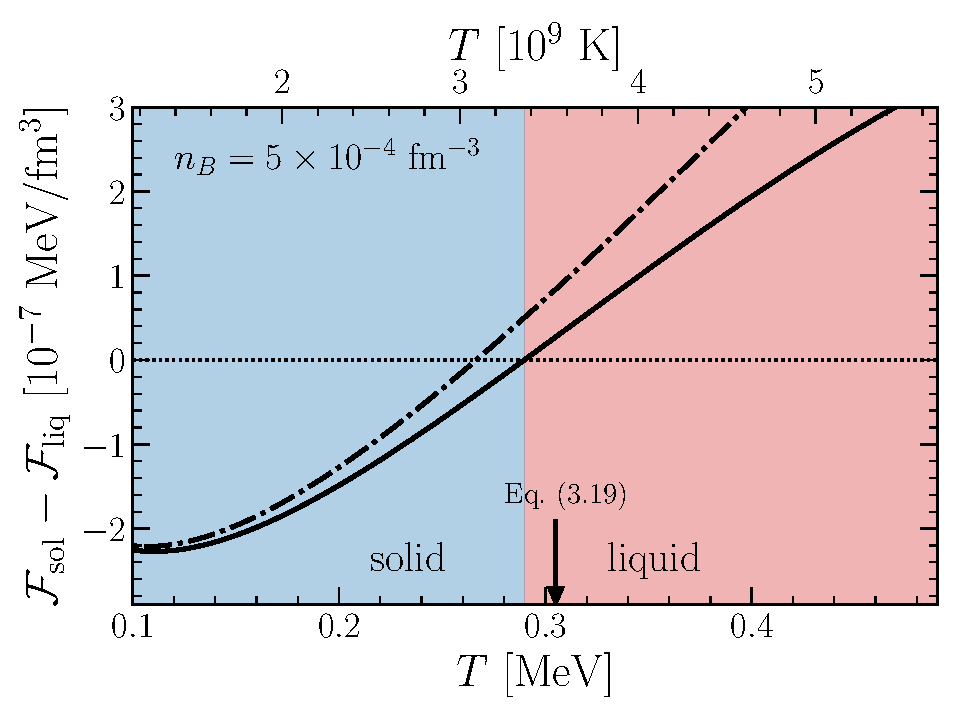
\includegraphics[width=0.9\linewidth]{figures/fliqsol.pdf}
  \end{center}
  \caption[Free energy density difference between liquid and solid phases
  versus temperature]{Variation with temperature $T$ of the free energy density
  difference between liquid and solid phases
$\mathcal{F}_{\text{sol}}-\mathcal{F}_{\text{liq}}$ for the optimal composition
$\bm{\theta_{\text{liq}}}$ at $n_B=5\times 10^{-4}$ 
\si{\per \cubic\femto\meter} (free neutron regime) with (solid line) and 
without (dashdotted line) the anharmonic contribution, Eq.~(\ref{eq:ah}), to 
the free energy in the solid phase, using BSk24 CLDM. The crystallization 
temperature obtained from Eq.~(\ref{eq:tmapprox}) is also 
indicated.}\label{fig:fliqsol}
\end{figure}

The condition of crystallization of a OCP with {associated composition 
$\bm{\theta}=\{A,Z,n_g\}$ and baryon density $n_B$ is defined as}
%
\begin{equation}
  \mathcal{F}_{\text{liq}}(\bm{\theta}, T_m) 
  = \mathcal{F}_{\text{sol}}(\bm{\theta}, T_m),\label{eq:tmocp}
\end{equation}
%
where $\mathcal{F}_\text{liq}$ and $\mathcal{F}_\text{sol}$ are the WS cell
free energy density in the liquid and solid phase, respectively.
The latter equation is equivalent to
%
\begin{equation}
  F_i^{\text{id}} + F_{ii,\text{liq}} = E_{zp} + F_{ii,\text{sol}},
\end{equation}
%
which shows that the Coulomb coupling parameter at melting
temperature $\Gamma_m$ does not depend on leading mass terms, but is fully
determined by the corrections that step in at 
finite temperature. Furthermore, those corrections are small in the vicinity of
the the crystallization temperature, making it difficult to estimate $\Gamma_m$ 
with precision. Still, several works estimate the Coulomb parameter to 
a constant $\Gamma_m \approx 175$~\cite{VanHorn1969,Haensel2007}. 
The crystallization temperature of a OCP at a given baryon density $n_B$ 
can then be approximated by inverting Eq.~(\ref{eq:gamma}), yielding
%
\begin{equation}
  T_m \simeq \frac{(Ze)^2}{k_B a_N \Gamma_m} \ \text{K},\label{eq:tmapprox}
\end{equation}
%
assuming the composition to be the same as in CCM. 
%
We proceed as in~\cite{Fantina2020} in order to precisely calculate the 
crystallization temperature. At each value of the baryon density $n_B$ and 
temperature $T$, the equilibrium composition is computed following the 
procedure detailed in Chapter 1. Specifically, we solve the coupled 
differential equations, Eqs.~(\ref{eq:ic1})-(\ref{eq:ic4}), using the 
expressions of $F_{i}^{\text{id}}$ and $F_{i}^{\text{int}}$ of the liquid 
phase, yielding the optimal liquid composition $\bm{\theta_{\text{liq}}}$ and 
the associated WS cell free energy density $\mathcal{F}_{\text{liq}}$. Then, 
for the same composition $\bm{\theta_{\text{liq}}}$, we calculate the free 
energy density assuming a solid phase 
$\mathcal{F}_{\text{sol}}(\bm{\theta_{\text{liq}}})$. The lowest temperature 
for which $\mathcal{F}_{\text{liq}} \geq \mathcal{F}_{\text{sol}}$ is 
identified as the crystallization temperature $T_m$ corresponding to the 
baryon density under study. The first guess for $T_m$ is obtained from the
application of Eq.~(\ref{eq:tmapprox}).

Fig.~\ref{fig:fliqsol} shows the variation with temperature of the free energy
difference $\mathcal{F}_{\text{sol}}-\mathcal{F}_{\text{liq}}$ at a given
baryon density $n_B = 5\times 10^{-4}$ for the BSk24 CLDM based on the 
metamodeling technique. The intersect of the solid line and zero marks
the crystallization temperature, $T_m = 0.29$ MeV, which is equivalent to $T_m
= (1.16\times 10^{10}) \times (0.29) = 3.36 \times 10^9$ K. We can observe that
the crystallization temperature is significantly lower if the 
anharmonic contribution to the free energy of the solid OCP is neglected 
(dashdotted line). This stresses the importance of the small thermal
corrections in the calculation. It is also seen that the effect of the 
anharmonic contribution becomes bigger with increasing temperature, and 
vanishes in case of strong coupling, that is in the zero-temperature limit. We
will show in Section~\ref{sec:ocrust_tm} that the simple expression 
Eq.~(\ref{eq:tmapprox}) gives a fairly good estimation of the 
crystallization temperature.

\subsection{Multicomponent Coulomb plasma in a liquid phase}\label{subsec:mcp}

The OCP approximation is expected to be reliable at the temperatures
typically encountered at low density in the crystallized crust, yet the 
very principle of statistical mechanics tells us that at finite temperature 
different configurations of the WS cell are realized for a same total density.
In the following, the nuclear distribution is included in an MCP approach at 
equilibrium, as in~\cite{Fantina2020,Carreau2020}. A 
particular attention is paid to the evaluation of the chemical potentials, as 
well as of the rearrangement term, which is required to ensure thermodynamic 
consistency. 

\subsubsection{Nuclear statistical equilibrium}

% introducing MCP formalism
The NS crust at a given depth in the star is supposed to contain different ion
species characterized by their mass and charge number $(A^{(j)},Z^{(j)})$, 
associated to different WS cells of volume $V_{WS}^{(j)}$, such that $p_j$ is 
the frequency of occurrence (or probability) of the component $(j)$, with 
$\sum_j p_j = 1$.
Thermodynamic quantities are defined in terms of the ion densities of the 
different species $n_N^{(j)}$, which are related to the probabilities $p_j$ 
through 
%
\begin{equation}
  n_N^{(j)}=\frac{p_j}{\langle V_{WS}\rangle}.\label{eq:nnj}
\end{equation}
%
where the average WS cell volume has been introduced,
%
\begin{equation}
  \langle V_{WS} \rangle = \sum_j p_j V_{WS}^{(j)},
\end{equation}
%
the notation $\langle\rangle$ indicating ensemble averages.
The different configurations $(A^{(j)},Z^{(j)})$ are associated with different
different baryon densities $n_B^{(j)}$, such that the total baryon density is
%
\begin{equation}
  n_B = \sum_j p_j n_B^{(j)}.
\end{equation}
%
Conversely, they share the same total pressure $P$ imposed by the hydrostatic 
equilibrium and the same background densities of electrons, $n_e^{(j)}=n_e$, 
and of free neutrons, $n_g^{(j)}=n_g$.
It is assumed that the charge neutrality is assured at the level of each cell,
implying that the proton density is the same in each cell, $n_p^{(j)}=n_p$, and
equal to the electron density, 
%
\begin{equation}
  n_e = n_p = \sum_j n_N^{(j)} Z^{(j)} =
  \frac{Z^{(j)}}{V_{WS}^{(j)}}.\label{eq:chargeneut}
\end{equation}

% energetics
The free energy density of the MCP is given by
%
\begin{equation}
  \mathcal{F} = \sum_j n_N^{(j)} F^{(j)},
\end{equation}
%
where $F^{(j)}$ is the free energy per ion of a single component $(j)$ defined 
in Eq.~(\ref{eq:fperion}).
The probabilities $p_j$ and ion densities $n_N^{(j)}$ are calculated such as to
maximize the thermodynamic potential in the canonical ensemble. 
Because of the chosen free energy decomposition, we can observe that the 
free neutron and electron contributions to the free energy density, 
respectively $\mathcal{F}_g$ and $\mathcal{F}_e$, do not depend on $n_N^{(j)}$,
%
\begin{equation}
  \mathcal{F}\left(\left\{n_N^{(j)}\right\}\right) 
  = \mathcal{F}_{i}\left(\left\{n_N^{(j)}\right\}\right) 
  + \mathcal{F}_g + \mathcal{F}_e,
\end{equation}
%
with
%
\begin{equation}
  \mathcal{F}_{i} = \sum_j n_N^{(j)} F_{i}^{(j)}.
\end{equation}
%
This means that the variation can be performed on the ion part only, yielding
%
\begin{eqnarray}
  d\mathcal{F}_{i} &=& \sum_j \left(F_{i}^{(j)} + n_N^{(j)} \frac{\partial
  F_{i}^{(j)}}{\partial n_N^{(j)}}\right)dn_N^{(j)} \notag\\
                     &=& \sum_j \left(F_{i}^{(j)} + k_B T + n_N^{(j)}
                     \frac{\partial F_i^{(j),\text{int}}}{\partial
                   n_N^{(j)}}\right)dn_N^{(j)} \notag\\
  &=& \sum_j \left(\Omega_{i}^{(j)} + k_B T \ln
  n_N^{(j)}\right)dn_N^{(j)},\label{eq:dfi}
\end{eqnarray}
%
where the single-ion canonical potential has been introduced,
%
\begin{equation}
  \Omega_{i}^{(j)} = M_{i}c^2 + k_B T\ln\frac{(\lambda^{(j)})}{g_s^{(j)}} 
  + F_i^{(j),\text{int}} 
  + n_N^{(j)} \frac{\partial F_i^{(j),\text{int}}}{\partial n_N^{(j)}}.
  \label{eq:omega}
\end{equation}
%
% discussion on the breaking of linear-mixing rule
A deviation to the linear-mixing rule (the hypothesis of uncorrelated WS 
cells) is observed in Eq.~(\ref{eq:omega}) due to the translational degree of 
freedom in the liquid phase~\cite{Gulminelli2015}, because within the MCP 
approach the center-of-mass position of each ion is not confined to the single 
cell volume $V_{WS}^{(j)}$ but can freely explore the whole volume. As a 
consequence, the average composition of the MCP does not coincide with the OCP 
optimal configuration in general.

% conservation laws
In Eq.~(\ref{eq:dfi}), the variations $dn_N^{(j)}$ are not independent because 
of the normalization of probabilities, and the baryon number and charge 
conservation laws:
%
\begin{eqnarray}
  \frac{1}{\langle V_{WS}\rangle} &=& \sum_j n_N^{(j)},\label{eq:normp}\\
  n_B - n_g &=& 
  \sum_j n_N^{(j)} A^{(j)}
  \left(1-\frac{n_g}{n_0^{(j)}}\right),\label{eq:barcons}\\
  n_p &=& \sum_j n_N^{(j)} Z^{(j)}\label{eq:charcons}.
\end{eqnarray}
%
We can identify the mass number associated to component $(j)$ in e-cluster 
representation $A_e^{(j)}$ in the right hand side of Eq.~(\ref{eq:barcons}).
Let us recall that in the regime of the outer crust, $n_g = 0$ fm$^{-3}$ thus
$A_e^{(j)} = A^{(j)}$. The average density of the ion $(j)$ $n_0^{(j)}$ is
obtained by solving numerically the equation corresponding to the pressure 
equilibrium between the ion and the gas (see~\ref{subsec:formalism} for the 
derivation),
%
\begin{equation}
  \frac{n_0^{(j)}}{A^{(j)}}\frac{\partial F_i^{(j)}} {\partial n_0^{(j)}} 
  = P_g,
\end{equation}
%
$P_g$ being the pressure of the neutron gas, whose expression is given in 
Eq.~(\ref{eq:phm}). As in~\cite{Grams2018}, the neutron gas density is taken to 
be the OCP solution, $n_g = n_g^{\text{OCP}}$.
% pj definition
The constraints Eqs.~(\ref{eq:normp})-(\ref{eq:charcons}) are taken into 
account by introducing the Lagrange multipliers $\alpha$, $\mu_n$, and $\mu_p$, 
leading to the following equations for the equilibrium densities $n_N^{(j)}$:
%
\begin{eqnarray}
  \sum_j \left(\Omega_{i}^{(j)} + k_B T \ln n_N^{(j)} 
  - \alpha\right)dn_N^{(j)} 
  - \mu_n \sum_j N_e^{(j)}dn_N^{(j)} - \mu_p \sum_j Z^{(j)} dn_N^{(j)}  
  = 0
\end{eqnarray}
%
with $N_e^{(j)} = A_e^{(j)} - Z^{(j)}$.
Considering independent variations, the solutions are given by
%
\begin{equation}
  p_j = \mathcal{A}\exp\left(-\frac{\tilde{\Omega}_{i}^{(j)}}{k_B
  T}\right),\label{eq:pj}
\end{equation}
%
with the normalization constant
%
\begin{equation}
  \mathcal{A} = \exp\left(\frac{\alpha}{k_B T}\right) = \sum_j
  \exp\left(-\frac{\tilde{\Omega}_{i}^{(j)}}{k_B T}\right).
\end{equation}
%
The single-ion grand-canonical potential reads
%
\begin{equation}
  \tilde{\Omega}_{i}^{(j)} = \Omega_{i}^{(j)} - \mu_n N_e^{(j)} -
  \mu_p Z^{(j)},
\end{equation}
%
where $\mu_n$ and $\mu_p$ physically correspond to the neutron and proton 
chemical potentials, respectively. Let us note that the rest-mass energies are 
included in the chemical potentials since they are contained in the ion 
free energy. 
% pj requires the evaluation of the rearrangement term as well as of the
%   neutron and proton chemical potentials
The calculation of the grand-canonical potential $\tilde{\Omega}_{i}^{(j)}$, 
entering the definition of the probabilities $p_j$, requires the 
evaluation of the chemical potentials $\mu_n$ and $\mu_p$, as well as of the 
rearrangement term
%
\begin{equation}
  \mathcal{R}^{(j)} = n_N^{(j)} 
  \frac{\partial F_i^{(j),\text{int}}}{\partial n_N^{(j)}},
\end{equation}
%
which are discussed thoroughly in~\ref{subsubsec:chempoteval}
and~\ref{subsubsec:rear}, respectively.

\subsubsection{Evaluation of the chemical
potentials}\label{subsubsec:chempoteval}

% expressions for mun and mup
For a given thermodynamic condition of pressure $P$ and temperature $T$, the
expression of the chemical potentials $\mu_n$ and $\mu_p$ can be derived from 
the well-known thermodynamic relation $\mathcal{F} + P = \mu_n n_n + \mu_p n_p 
+ \mu_e n_e$ together with the beta equilibrium condition $\mu_n = \mu_p + 
\mu_e$,
%
\begin{equation}
  \mu_n = \frac{\mathcal{F} + P}{n_B} \quad \text{and} \quad
  \mu_p = \mu_n - \frac{\mathcal{F}_e + P_e}{n_p},\label{eq:munmup}
\end{equation}
%
where the electron chemical potential and pressure, respectively $\mu_e$ and
$P_e$ have been introduced.
% how to normally solve the problem
The determination of the equilibrium probabilities $p_j$ within the complete 
NSE formalism therefore requires to solve a complex nonlinear system of coupled 
equations, which is obviously numerically costly. The implementation of 
the complete NSE was carried out in different studies in recent
years \edit{(see for example~\cite{Oertel2017,Burgio2018})}, but in those 
studies simplified nuclear functionals were adopted, \edit{baryon density} was 
imposed instead of the pressure, and the rearrangement term was neglected.

% perturbative implementation of NSE (update the chemical potentials)
We choose here to implement the NSE perturbatively, as proposed 
in~\cite{Grams2018}. 
The motivation for this option comes from the fact that the difference between
the chemical potentials in the OCP and MCP treatment were found to be very
small in~\cite{Gulminelli2015}. Moreover, in the recent work of Fantina 
\textit{et al.}, a very fast convergence of the chemical potentials is 
observed, along with a reduction of the computational time and an increase of
the numerical precision~\cite{Fantina2020}.
% explain how we proceed
We start by solving the OCP variational equations in order to get the 
equilibrium composition, which gives a first guess for the chemical potentials,
$\mu_n^{\text{OCP}}$ and $\mu_p^{\text{OCP}}$, via Eq.~(\ref{eq:munmup}). 
The probabilities $p_j$ can then be evaluated using Eq.~(\ref{eq:pj}), and an
improved estimation of the chemical potentials $\mu_n$ and $\mu_p$ is
calculated via
%
\begin{equation}
  \mu_n = \frac{\sum_j n_N^{(j)}F^{(j)}}{\sum_j n_N^{(j)}A_e^{(j)} + n_g} +
  \frac{P}{n_B} \quad \text{and} \quad
  y_p\mu_e = \frac{\sum_j n_N^{(j)}F_e^{(j)}}{\sum_j n_N^{(j)}A_e^{(j)} + n_g} 
  + \frac{P_e}{n_B},
\end{equation}
%
where the average proton fraction of the mixture $y_p=\langle
Z\rangle/(n_B\langle V_{WS}\rangle)$ has been introduced, with 
$\langle Z \rangle = \sum_j p_j Z^{(j)}$. The problem is thus solved by
iteration until the convergence of the chemical potentials is observed. The
convergence criterion is reasonably set to be $\Delta \mu_n < 10^{-9}$ MeV
between iterations.
We find that the number of iterations required to achieve convergence never 
exceeds 3. The reason is that the OCP result for $\mu_n$ and $\mu_p$ is 
already very close to the actual solutions for all pressures and 
temperatures explored in this work, thus confirming the results
of~\cite{Gulminelli2015}. Therefore, while we do solve the 
self-consistent problem by iterations in the regime of the outer crust 
to calculate the chemical potentials, the OCP estimation is safely kept in 
the free neutron regime so as to drastically reduce the computational cost. 
Indeed, in doing so the MCP calculation becomes equivalent to the much simpler 
OCP one.

\subsubsection{Evaluation of the rearrangement term}\label{subsubsec:rear}

At a given thermodynamic condition $(P,T)$, the rearrangement term entering 
Eq.~(\ref{eq:omega}) requires to be evaluated if one wants to compute the ion 
abundancies through Eq.~(\ref{eq:pj}).
As already discussed in~\cite{Grams2018,Fantina2020}, the rearrangement term 
arises from the self-consistency induced by the Coulomb part of the ion 
free energy. 
This stems from the fact that, due to the strong incompressibility of 
the electrons, the condition of charge neutrality has been imposed at the level 
of each cell, see Eq.~(\ref{eq:chargeneut}), in contrast with the baryon 
density $n_B$ that can fluctuate from cell to cell, see Eq.~(\ref{eq:barcons}). 
In consequence, any component of the free energy density that depends on the 
local cell proton density $n_p^{(j)} = n_p$ leads to a dependence on the local 
density $n_N^{(j)}$ through Eq.~(\ref{eq:chargeneut}). With our prescription 
for the WS cell free energy, this is only the case for the interacting part 
$F_i^{(j),\text{int}}$. We can therefore rewrite the rearrangement term of 
component $(j)$ as
%
\begin{eqnarray}
  \mathcal{R}^{(j)} 
  &=& n_N^{(j)} \left.\frac{\partial F_i^{(j),\text{int}}}{\partial
    n_N^{(j)}}\right|_{\{n_N^{(j)}\}_{i\neq j}}
    = n_N^{(j)} \frac{\partial F_i^{(j),\text{int}}}{\partial n_p}
    \frac{\partial n_p}{\partial n_N^{(j)}}\notag\\
  &=& n_N^{(j)} Z^{(j)} \frac{\partial F_i^{(j),\text{int}}}{\partial n_p}.
\end{eqnarray}
%
The complication of the self-consistent resolution of Eq.~(\ref{eq:pj}) can be 
avoided by imposing the most probable ion in the MCP mixture to coincide with 
the OCP result, if nonlinear mixing terms are omitted~\cite{Grams2018}. 
This approximation for the rearrangement term is justified by the principle of 
ensemble equivalence in the thermodynamic limit~\cite{Gulminelli2015}.

% the minimization
The maximum probability corresponds to the minimum of the single-ion
grand-canonical potential $\tilde{\Omega}_{i}$. We therefore minimize the 
single-ion grand-canonical potential with respect to $A$, $I=1-2Z/A$, and 
$n_0$ ($n_p$ and $n_g$ are fixed at a given thermodynamic condition), yielding 
the following nonlinear system of coupled equations:
%
\begin{eqnarray}
  \frac{n_0^2}{A}\left(\frac{\partial F_i}{\partial n_0} + \frac{\partial
  \mathcal{R}}{\partial n_0}\right) &=& P_g\label{eq:r1}\\
  \frac{2}{A}\left(\frac{\partial F_i}{\partial I} + \frac{\partial
  \mathcal{R}}{\partial I}\right) &=& \mu_n - \mu_p\label{eq:r2}\\
  \frac{\partial F_i}{\partial A} + \frac{\partial \mathcal{R}}{\partial A} +
  \frac{1-I}{A}\left(\frac{\partial F_i}{\partial I} + \frac{\partial
  \mathcal{R}}{\partial I}\right) &=& \mu_n - \frac{P_g}{n_0},\label{eq:r3}
\end{eqnarray}
%
where the partial derivatives are calculated at the values corresponding to 
the equilibrium OCP solution, with nonlinear mixing terms being excluded.
%
The comparison of Eqs.~(\ref{eq:r1})-(\ref{eq:r3}) with
Eqs.~(\ref{eq:ic2})-(\ref{eq:ic4}) indicates that $\mathcal{R}^{(j)}$ should 
not depend on $n_0^{(j)}$, meaning that $R^{(j)}=R^{(j)}(A^{(j)},Z^{(j)})$. In 
addition, the rearrangement term should verify the following equation at the 
OCP solution:
%
\begin{equation}
  \frac{1-I}{A}\frac{\partial \mathcal{R}}{\partial I} = -\frac{\partial
  \mathcal{R}}{\partial A},
\end{equation}
%
which is satisfied if $R^{(j)}$ linearly depends on 
$Z^{(j)} = A^{(j)} (1-I^{(j)})/2$. Our final expression for the rearrangement 
term is therefore
%
\begin{equation}
  \mathcal{R}^{(j)} \simeq Z^{(j)} \left\langle \langle n_N^{(j)}\rangle 
    \frac{\partial F_i^{(j),\text{int}}}{\partial n_p}\right\rangle_j
  = \frac{Z^{(j)}}{V_{WS}^{\text{OCP}}}
  \left.\frac{\partial F_i^{\text{int}}}{\partial
    n_p}\right|_{\text{OCP}},\label{eq:rear}
\end{equation}
%
where $V_{WS}^{\text{OCP}}$ is the equilibrium OCP cell volume, and the
derivative is evaluated numerically at the OCP solution.

\subsection{Nuclear free energy functional in the free neutron 
regime}\label{subsec:freeenfunctional}

% in the regime of the outer crust, we make use of exp data
As previously discussed in Chapter 1, in the regime of the outer crust we use 
the present day knowledge on experimental masses of neutron rich 
nuclei~\cite{Huang2017,Welker2017}, combined with state-of-the-art 
microscopic HFB theoretical mass tables~\cite{Goriely2013}. 
In principle, at finite temperature an entropy term should be added to the mass
table leading to a temperature dependent degeneracy replacing the ground state
spin degeneracy $g_s$. However, the crystallization temperature is so low in
the outer crust that we make the approximation that the nuclei are in their
ground state. 
The ion mass $M_{i}$ in the outer crust is therefore simply calculated using 
Eq.~(\ref{eq:ionmass}).

% ion mass in the inner crust
In the regime of the inner crust, $n_B \gtrsim 2.6 \times 10^{-4}$ fm$^{-3}$, 
we have seen that the ions are immersed in a neutron gas, whose free energy 
density $\mathcal{F}_g$ enters the expression of the ion mass in the e-cluster 
representation,
%
\begin{equation}
  M_{i}^{(j)} c^2 = (A^{(j)} - Z^{(j)})m_n c^2 + Z^{(j)} m_p c^2 
  + F_{cl}^{(j)} - \frac{A^{(j)}}{n_0^{(j)}}(\mathcal{F}_g + n_g m_n c^2),
\end{equation}
%
where $F_{cl}^{(j)}$ represents the nuclear free energy, including the
contribution of the resonant and continuum excited states.
In the range of densities corresponding to the free neutron regime, the 
clusters are by definition above the drip line, so that experimental data are 
not available. As a consequence, the modeling of $F_{cl}^{(j)}$ is required.

% plan
In the following, we first recall the simple case of free FG before
deriving the expressions required to describe to the ambient neutron gas at 
finite temperature. 
We then give the expressions of the different quantities entering the 
expression of the smooth part of the nuclear free energy functional 
$F_{cl}^{(j)}$. The temperature dependence of shell corrections and its effect 
on the crystallization temperature is investigated in~\ref{subsec:shtemp}.

\subsubsection{Thermodynamics of nuclear matter}

Let us first consider a collection of noninteracting fermions. In the 
grand-canonical ensemble, it obeys Fermi-Dirac statistics and the average 
number of fermions occupying a single-particle state $i$ is given by the 
Fermi-Dirac distribution, 
%
\begin{equation}
  \langle n_i \rangle 
  = \left[1+\exp\left(\frac{e_i-\mu}{k_B T}\right)\right]^{-1},
\end{equation}
%
where $e_i$ is the energy of the single-particle state $i$, and $\mu$ is the
total chemical potential.
At the thermodynamic limit, the sum over states $i$ is replaced by an integral
over the energy, thus the Fermi-Dirac function that describe the
occupation rate of state of given energy $e$ is introduced,
%
\begin{equation}
  f_{\text{FD}}(e, T, \mu) 
  = \left[1+\exp\left(\frac{e-\mu}{k_B T}\right)\right]^{-1}.\label{eq:fFD}
\end{equation}
%
When replacing the sum by an integral, one needs to introduce the density of
energy states $\rho(e)$. For a spinless free particle of energy $e=\hbar^2 
k^2/(2m)$, the density of states is given by $\rho(\vec{k}) =
\frac{V}{(2\pi)^3}$, with $k$ the wave vector and $V$ the volume. Using the 
relation $\rho(\vec{k})d^3k = \rho(e)de$, one obtains
%
\begin{equation}
  \rho(e) = g\frac{V}{4\pi^2}\left(\frac{2m}{\hbar^2}\right)^{3/2}\sqrt{e},
\end{equation}
%
where the spin degeneracy $g=2s+1$ (for fermions, $s=1/2$) has been introduced, 
and $m$ is the mass of a particle.
At the thermodynamic limit, that is if we consider a huge number of particles
at a given temperature $T$ so that a large number of states are occupied, all
ensembles are equivalent. This means that we can use the expressions of 
the grand-canonical ensemble to calculate for instance the exact number of 
particles and the energy, respectively
%
\begin{equation}
  N = \sum_i\langle n_i\rangle \simeq \int_0^\infty
  \rho(e)f_{\text{FD}}(e)de
  \quad \text{and} \quad 
  E \simeq \int_0^\infty e \rho(e) f_{\text{FD}}(e)de.\label{eq:stats_N}
\end{equation}
%

% zero temperature
At zero temperature, states are populated up to the Fermi energy $\mu(T=0) =
e_F$. Indeed, $f_{\text{FD}} = 1$ for $e < \mu$, otherwise $f_{\text{FD}} = 0$, 
which allows us to rewrite Eq.~(\ref{eq:stats_N}) as
%
\begin{equation}
  N(T=0) = \int_0^{e_F} de\rho(e),
\end{equation}
%
yielding the expression of the Fermi energy,
%
\begin{equation}
  e_F = \frac{\hbar^2}{2m}\left(3\pi^2\frac{N(T=0)}{V}\right)^{2/3} =
  \frac{\hbar^2 k_F^2}{2m},\label{eq:eF}
\end{equation}
%
with $k_F=(3\pi^2N(T=0)/V)^{1/3}$ the Fermi wave vector.
At $T=0$ K, the free energy is simply equivalent to the energy:
%
\begin{equation}
  F(T=0) = E(T=0) = \int_0^{e_F} e\rho(e)de = \frac{3}{5}Ne_F.
\end{equation}
%

At nonzero temperature, the calculation of thermodynamic properties of a free
FG generally requires the numerical evaluation of Fermi integrals,
%
\begin{equation}
  F_\nu(u) = \frac{1}{\Gamma(\nu+1)}\int_0^\infty\frac{t^\nu}{1+\exp(t-u)}dt,
\end{equation}
%
where $\Gamma(\nu) = (\nu-1)!$ is the gamma function.
It is however useful to apply Sommerfeld development in the limit $T \ll
e_F$ -- which is satisfied in the range of temperatures explored in our work -- 
in order to derive analytical formulas. In that case, we can obtain the
expression of the chemical potential from $N=\int_0^\infty
\rho(e)f_{\text{FD}}(e)de$, assuming that $\mu=e_F(1+\alpha T^2)$. By
identifying terms scaling as $T^2$, we get
%
\begin{equation}
  \mu = e_F\left[1 - \frac{\pi^2}{12}\left(\frac{T}{e_F}\right)^2\right].
\end{equation}
%
We can proceed in the same manner to calculate the energy at finite
temperature and the entropy, respectively
%
\begin{equation}
  E = \frac{3}{5} N e_F 
  \left[1+\frac{5\pi^2}{12}\left(\frac{T}{e_F}\right)^2\right] \quad \text{and}
  \quad S = \frac{\pi^2}{2}N\frac{T}{e_F},
\end{equation}
%
which finally gives, using the thermodynamic relation $F=E-TS$, the expression
of the free energy of a nonrelativistic free FG,
%
\begin{equation}
  F = \frac{3}{5} N e_F
  \left[1-\frac{5\pi^2}{12}\left(\frac{T}{e_F}\right)^2\right].
\end{equation}
%

In the framework of the finite temperature self-consistent mean-field
approximation, it is possible to show that those results can still be used in 
the case of a huge number of interacting fermions in a infinite volume at a 
finite density, that is for infinite nuclear matter~\cite{Vautherin1996}. 
The energy density $\mathcal{H} = \mathcal{K} + \mathcal{V}$ for this 
idealized system can be derived from an
effective functional, and is often decomposed into a kinetic term and a 
contribution due to the nuclear interactions, respectively $\mathcal{K}$ and 
$\mathcal{V}$, which both in infinite homogeneous nuclear matter only depend on
local densities $n_q$.
As discussed in~\ref{subsubsec:hnm}, the Landau effective mass $m_q^*$ of 
species $q$ is usually introduced to regroup in a single term of kinetic 
energy the momentum dependence of the mean field,
%
\begin{equation}
  \frac{\hbar^2 k_q^2}{2m_q^*} = \frac{\hbar^2 k_q^2}{2m_q} +
  U_{\text{eff}}(k_q).
\end{equation}
%
In the grand-canonical ensemble, the occupation rate of state of given energy
$e_q$ for interacting fermions reads
%
\begin{equation}
  f_q(e_q+U_q, T, \mu_q) 
  = \left[1+\exp\left(\frac{e_q + U_q - \mu_q}{k_B T}\right)\right]^{-1},
\end{equation}
%
where $e_q + U_q = \hbar^2 k_q^2/(2m_q^*) + U_q$ is the single-particle energy
of species $q$, $U_q = \partial\mathcal{H}/\partial n_q$ being the local mean
field potential, which is given in the metamodel by ($q=n,p$)
%
\begin{eqnarray}
  U_q &=& v_{MM}(n,\delta) + \frac{1+3x}{3}\left(\frac{\partial
  v_{MM}}{\partial x}\right)_{\delta}
  + (\tau_3 - \delta) 
  \left(\frac{\partial v_{MM}}{\partial \delta}\right)_x\notag\\
      &&+ (1+3x)\sum_{l=n,p}\frac{3}{5}\frac{1+\tau_{3,l}\delta}{2}
      e_{F,l}\left[1-\frac{5\pi^2}{12}\left(\frac{T}{e_{F,l}}\right)^2\right]
      \notag\\
      &&\times \frac{m_l^*}{m} \left[
        \kappa_{sat}+\tau_{3,l} \kappa_{sym} \left(\delta
        + \frac{\tau_3-\delta}{1+3x}\right)
    \right],
\end{eqnarray}
%
with $\tau_{3,l} = 1$ ($\tau_{3,l} = -1$) for $l=n$ ($l=p$). The expressions of
the potential energy $v_{MM}$ and effective masses are given 
in~\ref{subsubsec:hnm}. The simple case of free FG is recovered by 
introducing the effective chemical potential $\tilde{\mu}_q = \mu_q - U_q$,
yielding the free energy per particle of nuclear matter,
%
\begin{equation}
  f_{HM}(n,\delta,T) = \sum_{q=n,p}
  \frac{3}{5}\frac{1+\tau_3\delta}{2}e_{F,q}\left[
  1-\frac{5\pi^2}{12}\left(\frac{T}{e_{F,q}}\right)^2\right] +
  v_{MM}(n,\delta),\label{eq:freehm}
\end{equation}
%
which enters the expression of the neutron gas free energy, $\mathcal{F}_g =
n_g f_{HM}(n_g,1,T)$. {It is important to stress that the Fermi energy 
  $e_F,q$ contains the effective mass in the above equation, contrary to
Eq.~(\ref{eq:eF}).}
Let us note that the chemical potential does not include the rest mass energy 
in the above expressions. 
We can remark the well-known fact that in the mean-field approximation the
temperature affects only the occupation of the single-particle levels, and not
the value of the single-particle energies. As a consequence, if the density is
homogeneous, $n_q = cst$, the potential part of the free energy is temperature
independent, and the same expressions as in Chapter 1 are obtained. An effect
of the functional on the finite temperature properties however is expected,
because the interaction enters the kinetic part via the effective mass.

\subsubsection{Energetics of clusters at finite temperature in the CLD
approximation}

Within the CLD approximation, the nuclear free energy $F_{cl}$ at temperature 
$T$ of a cluster of mass number $A$, isospin asymmetry $I$, and average density 
$n_0$, can be decomposed into a bulk, surface and Coulomb part as
%
\begin{equation}
  F_{cl}^{\text(CLD)} = A f_{HM}(n_0,I,T) + F_{surf} + F_{curv} + F_{Coul},
\end{equation}
%
where $f_{HM}(n_0, I, T)$ represents the free energy per baryon of bulk nuclear
matter, which is calculated using Eq.~(\ref{eq:freehm}).
The expressions used for the surface and curvature free energy are given
in Eqs.~(\ref{eq:esurf}) and~(\ref{eq:ecurv}) respectively, with the exception
of the surface tension, Eq.~(\ref{eq:sigma}) whose expression is modified with 
respect to the zero temperature case in order to effectively account for the 
excitation of surface modes:
%
\begin{equation}
  \sigma(I,T) = \sigma(I, T=0)h(T), 
\end{equation}
%
with $h(T>T_c) = 0$ and $h(T \leq T_c) = [1-(T/T_c)^2]^2$ (see Eq.~(2.31)
of~\cite{Lattimer1991}).
However, because the critical temperature $T_c$ is of the order of 
$T_c \approx 1.75 \times 10^{11}$ K and the crystallization temperature is 
lower than $10^{10}$ K in the inner crust~\cite{Haensel2007}, $h\approx 1$ and 
the excitation of surface modes can be neglected.
Assuming spherical clusters, we write the Coulomb energy as
%
\begin{equation}
  F_{Coul} = \frac{3}{5}\frac{e^2}{r_0^2}\frac{Z^2}{A^{1/3}}.
\end{equation}
%

We limit ourselves to the empirical parameters 
associated to four different functionals of the BSk family taken 
from~\cite{Goriely2013}: BSk22, BSk24, BSk25, and BSk26.
We choose these models because they all provide excellent fits to the 
AME2016 \cite{Huang2017}, are compatible both with \textit{ab initio} and NS 
mass constraints, and explore a relatively large domain in the symmetry energy 
parameters (consistent with existing experimental constraints), which 
constitute the most important part of the EoS 
uncertainty~\cite{Pearson2014,Pearson2018}. Moreover, for each functional, 
surface and curvature parameters can be fitted to the ETF 
results~\cite{Pearson2019}, and the corresponding Strutinsky shell corrections, 
which are tabulated in~\cite{Pearson2018}, can be added on top of the CLD free 
energy, see~\ref{subsec:strutinsky} and~\ref{subsec:shtemp}.
Another motivation is that full mass tables obtained by deformed HFB 
calculations have been published for these models~\cite{Xu2013} and can 
therefore be used in the regime of the outer crust as a
complement to experimental masses~\cite{Fantina2020}. 
However, some different models, not considered in~\cite{Fantina2020}, are also
considered in order to appreciate the model dependence of the results. A full
Bayesian study at finite temperature is left for future work.

\section{Study of the outer crust at crystallization}\label{sec:ocrust_tm}

In this section, we present the results for the outer crust at finite
temperature, and more specifically at crystallization.
% what is included by default
Unless explicitly stated, all thermal corrections introduced in
Section~\ref{sec:modelcrusttemp} are included in the ion free energy.
% exp data when available
We made use of experimental masses from AME2016 \cite{Huang2017} when 
available, apart from the mass excesses of $^{77-79}$Cu which are better 
constrained in~\cite{Welker2017}.
{The calculations are performed independently of those 
  of Fantina \textit{et al.}~\cite{Fantina2020}, observing a perfect 
  agreement between the two studies shows that the numerical code of this 
  work is under control.}

The crystallization temperature of a OCP is calculated throughout the outer
crust in~\ref{subsec:tm_ocrust}. In~\ref{subsec:compo_ocrust_tm}, the
equilibrium composition of the MCP at crystallization is presented, and 
deviations from the ground-state composition are investigated. The variation 
with pressure of the impurity parameter is analyzed 
in~\ref{subsec:qimp_ocrust}. Finally, the fraction of odd nuclei present in the 
outer crust at crystallization is computed in~\ref{subsec:odd_ocrust}.

\subsection{Crystallization temperature}\label{subsec:tm_ocrust}

\begin{figure}[!t]
  \begin{center}
    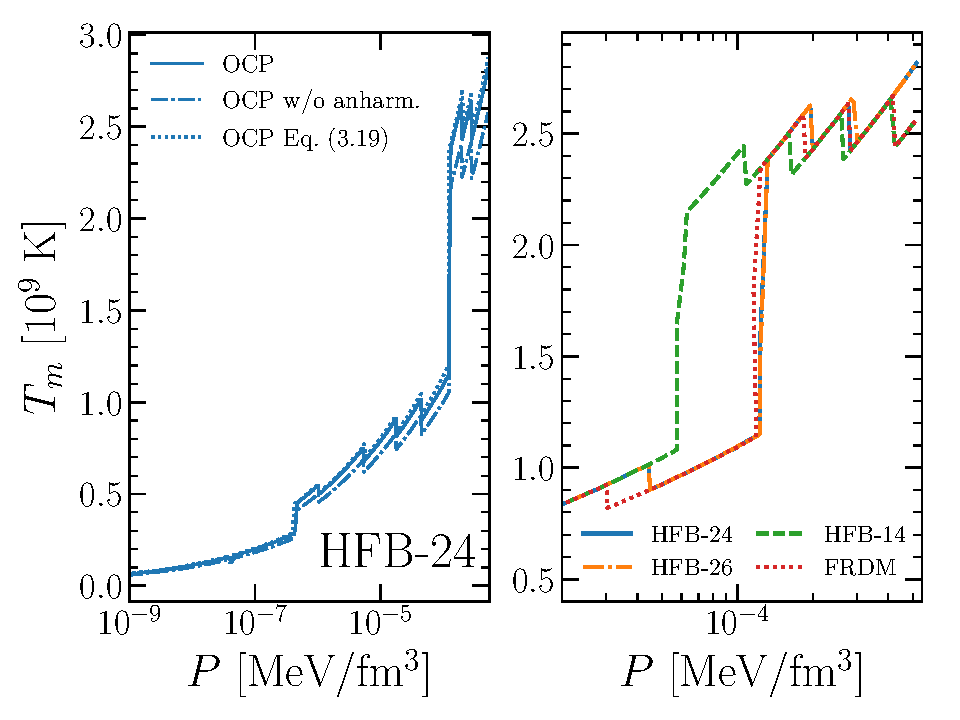
\includegraphics[width=0.9\linewidth]{figures/tm_ocrust.pdf}
  \end{center}
  \caption[Crystallization temperature versus pressure for the one-component 
  plasma in the outer crust]{Crystallization temperature $T_m$ as a function of
    pressure $P$ for the OCP in the outer crust. The left panel shows $T_m$ 
    for the  OCP with all corrections included (solid line), without 
    taking into account the anharmonic contribution (dashdotted line), and 
    the result obtained from Eq.~(\ref{eq:tmapprox}) (dotted line). 
    Experimental data are supplemented with masses from the microscopic HFB-24 
    theoretical mass table~\cite{Goriely2013}. 
    The right panel shows $T_m$ in the bottom layers of the outer crust for 
    four selected models: HFB-24 (solid blue line), HFB-26~\cite{Goriely2013}
    (dashdotted orange line), HFB-14~\cite{Goriely2007} (dashed green line), 
  and FRDM~\cite{Moller1995} (dotted red line).}\label{fig:tm_ocrust}
\end{figure}

% LEFT PANEL
The left panel of Fig.~\ref{fig:tm_ocrust} shows the crystallization
temperature as a function of the pressure in the outer crust, as obtained in 
the OCP approximation, Eq.~(\ref{eq:tmocp}). 
Experimental masses are supplemented with the microscopic HFB-24 theoretical 
mass table~\cite{Goriely2013}. 
It is seen that the crystallization temperature is overall an increasing
function of the pressure in the outer crust, and ranges from approximately 
$5\times 10^7$ K ($4$ keV) at very low pressure to $2.8\times 10^9$ K ($240$ 
keV) close to the neutron-drip point.
As one could have expected from the quadratic dependence on $Z$ observed in 
Eq.~(\ref{eq:tmapprox}), we can see that the effect of shell structure on the 
crystallization temperature is very important. Indeed, each change in the 
equilibrium OCP composition results in an abrupt change in $T_m$, that is 
clearly noticeable in Fig.~\ref{fig:tm_ocrust}. In particular, the fact that 
the curve of the crystallization temperature is very steep in the vicinity of 
$P=1.2\times 10^{-4}$ MeV/fm$^3$, with $T_m$ rapidly increasing from 
$1.2\times 10^9$ K to $2.4\times 10^9$ K, can be attributed to the
transition from $N=50$ to $N=82$, observed in Fig.~\ref{fig:ocrust_model}.
The importance of the anharmonic contribution to the ion free energy of a 
solid OCP, already investigated in Fig.~\ref{fig:fliqsol}, can be appreciated 
in the left panel of Fig.~\ref{fig:tm_ocrust} by comparing the solid and 
dashdotted blue lines. We recover the result of~\cite{Fantina2020} that the 
crystallization temperature is quite sensitive to the anharmonic contribution.
We find that not accounting for this thermal correction induces an error on 
$T_m$ of the order of $10\%$ in the range of pressure corresponding to the 
outer crust.
The dotted blue line shows the result of the approximation 
Eq.~(\ref{eq:tmapprox}). It is seen that one can obtain a very good 
estimation of the crystallization temperature for all pressures in the outer 
crust by using this approximation, which indicates that the crystallized 
composition (at $T=T_m$) is very similar to that at $T=0$ K. This is discussed 
in detail in~\ref{subsec:compo_ocrust_tm}. The fact that 
Eq.~(\ref{eq:tmapprox}) systematically but only slightly overestimates the 
crystallization temperature justifies its use for getting a first estimate so 
as to reduce the computational time. 

% RIGHT PANEL
The model dependence of the crystallization temperature of a OCP is illustrated 
in the right panel of Fig.~\ref{fig:tm_ocrust}, where $T_m$ is represented as a
function of $P$ for four different models that supplement experimental data:
HFB-24, HFB-26~\cite{Goriely2013}, HFB-14~\cite{Goriely2007}, and
FRDM~\cite{Moller1995}. 
As for the equilibrium composition of CCM, see Fig.~\ref{fig:ocrust_model}, the 
crystallization temperature becomes sensitive to the model from $P \approx 
3\times 10^{-5}$ MeV/fm$^{3}$, due to nuclei being so neutron rich that 
experimental masses are not available. We can see that the results are very
close for HFB-24, HFB-26, and FRDM, even if these models considerably differ in
their mass prediction, and HFB-24 and HFB-26 correspond to very different EoS.
This finding shows once again the importance of the small thermal corrections 
in the calculation, which determine in first approximation the crystallization
temperature independently of the mass model.

\subsection{Equilibrium composition}\label{subsec:compo_ocrust_tm}

\begin{figure}[!t]
  \begin{center}
    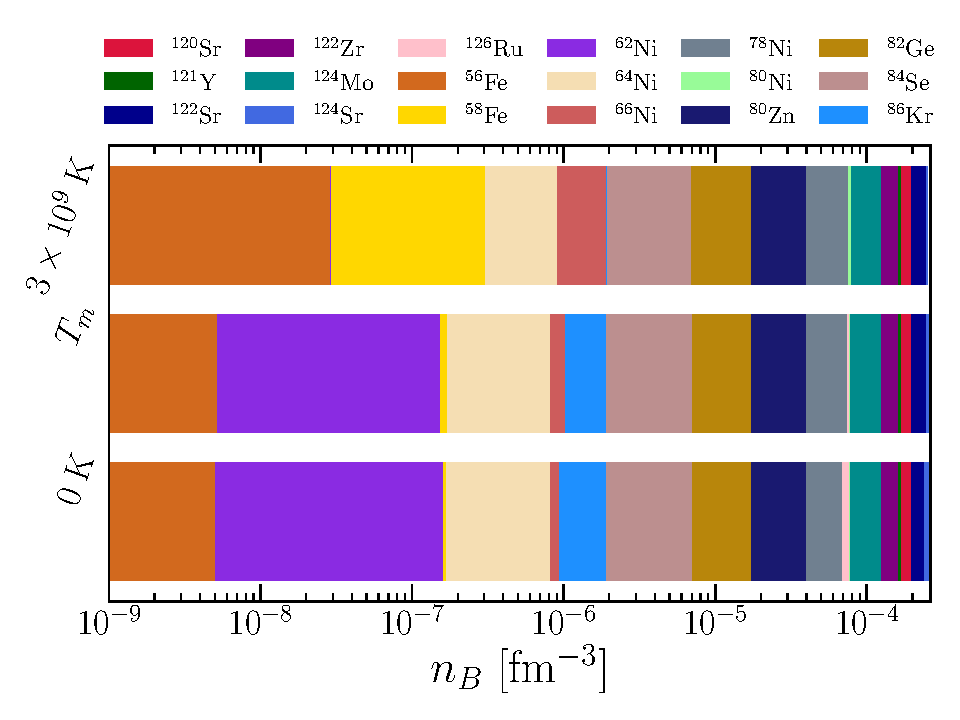
\includegraphics[width=\linewidth]{figures/ocrust_compo_vs_temp.pdf}
  \end{center}
  \caption[Equilibrium OCP composition versus baryon density in the outer crust 
  at finite temperature]{Equilibrium composition of a OCP as a function of 
    baryon density $n_B$ in the outer crust at $T=0$ \si{\kelvin}, $T=T_m$, and 
    $T=3\times 10^9$ \si{\kelvin}. 
  Experimental data are supplemented with masses from the microscopic HFB-24 
  theoretical mass table~\cite{Goriely2013}.}\label{fig:ocrust_compo_vs_temp}
\end{figure}

The crystallization temperature in the outer crust does not exceed $\approx
0.25$ MeV, which is very low from the nuclear physics point of view. Hence, one
can ask whether the composition at crystallization is different to that of
CCM, presented in Section~\ref{sec:ocrust_gs}.
Fig.~\ref{fig:ocrust_compo_vs_temp} shows the equilibrium composition of a OCP
as a function of the baryon density $n_B$ in the regime of the outer crust for
two different temperatures: $T=0$ K (CCM) and $T=3\times 10^9$ K, and at 
crystallization, $T=T_m$. We make use of the microscopic HFB-24 theoretical 
mass table to complement the experimental data.
Let us notice that for all densities encountered in the outer crust, nonlinear 
mixing effects are so small that the equilibrium nucleus obtained within OCP 
approximation coincides with the most probable ion in the MCP mixture.
% discuss differences between t=0 and t=tm
We find that the difference between $T=0$ K and $T=T_m$ is very small and 
hardly visible in the figure. The exact same sequence of layers is observed in 
the two cases, only the transition densities being slightly different.
This shows that the CCM hypothesis gives an accurate description of the 
composition of the outer crust at crystallization.
% observations at larger temperatures
Significant deviations with respect to the results at $T=0$ K and $T=T_m$ are 
observed at $T=3\times 10^9$ K, which is above the crystallization temperature
in the outer crust. In particular, the layers of $^{62}$Ni and $^{86}$Kr are 
not recovered, and $^{80}$Ni is favored over $^{126}$Ru around $n_B \approx 
8\times 10^{-5}$ fm$^{-3}$. 
These results could have some implications in NS cooling simulations,
where the approximation is often made that the composition at finite
temperature is the same as at zero temperature~\cite{Fortin2010}. A possible
relevance to the physics of (cold) NS cannot be excluded either, since the ion
distribution could be frozen at some temperature $T_f>T_m$ considering the
present uncertainties on timescales relative to NS cooling~\cite{Goriely2011}.
This point deserves further investigations.

\begin{figure}[!t]
  \begin{center}
    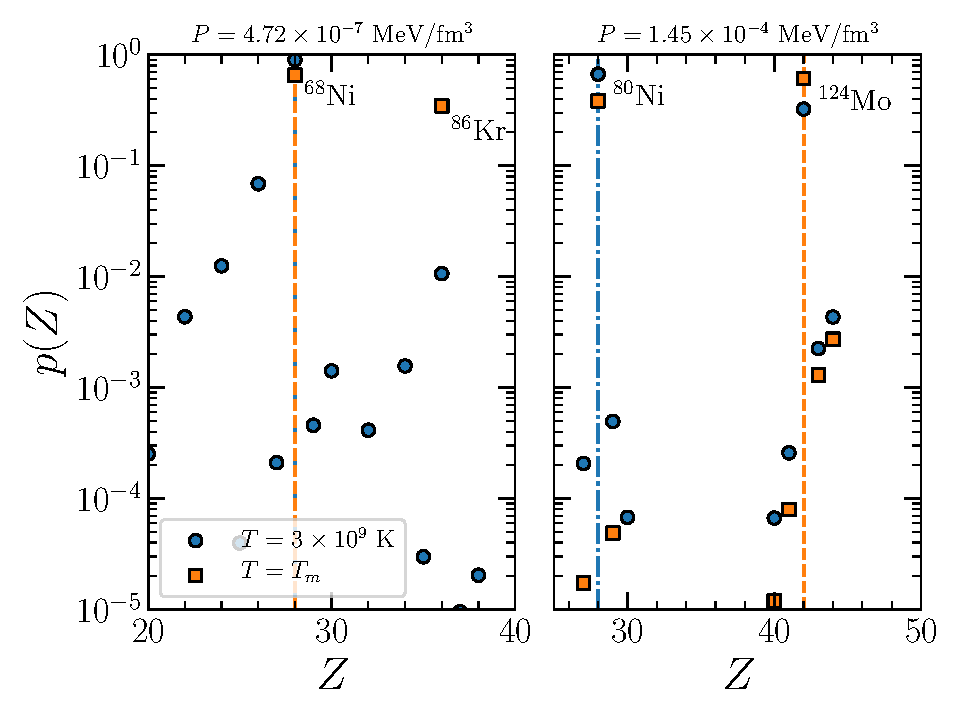
\includegraphics[width=0.9\linewidth]{figures/pj_ocrust.pdf}
  \end{center}
  \caption[Normalized probability distribution of the atomic number $Z$ in the 
  outer-crust regime]{Normalized 
    probability distribution 
    $p(Z)$ for $P=4.72\times 10^{-7}$ \si{\MeV \per \cubic\femto\meter} (left 
    panel) and $P=1.45\times 
    10^{-4}$ \si{\MeV \per \cubic\femto\meter} (right panel), at 
    $T=3\times 10^9$ \si{\kelvin} (blue circles) and 
    $T=T_m$ (orange squares). The blue dashdotted and orange dashed vertical 
    lines indicate the OCP solution at $T=3\times 10^9$ \si{\kelvin} and 
    $T=T_m$, respectively.
    Experimental data are supplemented with masses from the microscopic 
    HFB-24 theoretical mass table~\cite{Goriely2013}. 
    Figure inspired from~\cite{Fantina2020}.}\label{fig:pj_ocrust}
\end{figure}

\begin{figure}[!t]
  \begin{center}
    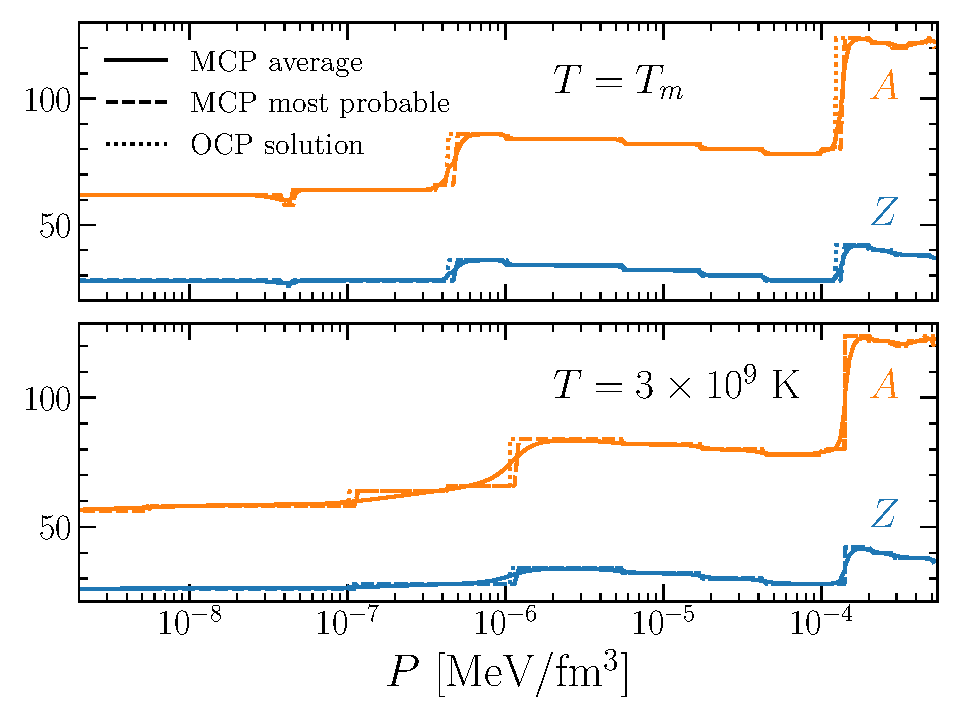
\includegraphics[width=0.9\linewidth]{figures/compo_mcp_ocrust.pdf}
  \end{center}
  \caption[Equilibrium composition of the multicomponent plasma versus pressure
  in the outer-crust regime]{
    Average (solid lines) and most probable values (dashed lines) of the charge 
    number $Z$ (blue lines) and mass number $A$ (orange lines) in the MCP 
    mixture as a function of pressure in the regime of the outer crust at 
    $T=T_m$ (upper panel) and $T=3\times 10^9$ \si{\kelvin} (lower panel). 
    The OCP solution is represented in dotted lines.
    Experimental data are supplemented with masses from the microscopic 
    HFB-24 theoretical mass table~\cite{Goriely2013}. 
  Figure inspired from~\cite{Fantina2020}.}\label{fig:compo_mcp_ocrust}
\end{figure}

The normalized probability distribution $p(Z)$ of the MCP mixture is 
represented in Fig.~\ref{fig:pj_ocrust} for different thermodynamic conditions 
relevant for the regime of the outer crust: $P = 4.72\times 10^{-7}$ MeV/fm$^3$
(left panel) and $P=1.45\times 10^{-4}$ MeV/fm$^3$ (right panel). For both 
selected values of pressure, we plot the distribution for $T=3\times
10^9$ K (blue circles) and for the crystallization temperature $T=T_m$ 
calculated within the OCP approximation (orange squares).
For each selected thermodynamic condition, it is observed that the most
probable $Z$ in the MCP mixture coincides with the OCP solution represented by 
a vertical line.
At low pressure, the crystallization temperature is small and consequently only 
very few configurations occur. This can be seen in the left
panel of the figure, $P = 4.72\times 10^{-7}$ MeV/fm$^3$, where only $Z=28$
($p(^{66}\text{Ni}) = 0.65$) and $Z=36$ ($p(^{86}\text{Kr})=0.35$) are 
associated to nonnegligible probabilities. This contrasts with the 
distribution calculated 
at $T=3\times 10^9$ K for the same value of pressure, for which a large number 
of configurations are found with $p(Z) > 10^{-5}$. Still, at this temperature 
the distribution is strongly peaked at $Z=28$, while for $T=T_m$ the 
distribution is bimodal. 
In the right panel of Fig.~\ref{fig:pj_ocrust}, a bimodal behavior is also 
clearly exhibited around $Z=28$ and $Z=42$, respectively corresponding to 
$^{80}$Ni and $^{124}$Mo, in the vicinity of $P = 1.45\times 10^{-4}$ 
MeV/fm$^3$, where the curve of the crystallization temperature becomes very 
steep, see Fig.~\ref{fig:tm_ocrust}. 
While $^{124}$Mo is favored over $^{80}$Ni at high temperature,
it turns out that the most probable nucleus changes to $^{80}$Ni as the
temperature is decreased, and ultimately corresponds to the most probable
nucleus at the crystallization temperature. The same feature is observed for 
the OCP solution.

Fig.~\ref{fig:compo_mcp_ocrust} shows the equilibrium composition of the MCP as
a function of pressure in the regime of the outer crust at the crystallization
temperature (upper panel) and at $T=3\times 10^9$ K (lower panel). At $T=T_m$, 
it is seen that the average equilibrium values $\langle Z\rangle$ and $\langle
A\rangle$ (solid blue and orange lines, respectively) coincides almost 
perfectly with the OCP solution (dotted blue and orange lines), apart in the
vicinity of $P=4.5\times 10^{-7}$ MeV/fm$^3$ and $P=1.5\times 10^{-4}$
MeV/fm$^3$, where the distribution $p(Z)$ exhibits a bimodal character, as
observed in Fig.~\ref{fig:pj_ocrust}. This results in the softening of the 
shell effects, which is even more striking at $T=3\times 10^9$ K. Those 
deviations from the OCP approximation are reflected in the Coulomb coupling 
parameter, which exhibits spikes and can be as high as $\approx 330$ at the
crystallization temperature, see Fig.~4 of~\cite{Fantina2020}.

\subsection{Impurity parameter}\label{subsec:qimp_ocrust}

% definition
Once the abundancies of the different ions are computed via Eq.~(\ref{eq:pj}), 
the so-called impurity parameter of the solid crust, which represents the 
variance of the ionic charge distribution, can be evaluated. It is defined
as~\cite{Meisel2018}
%
\begin{equation}
  Q_{\text{imp}} = \sum_j p(Z^{(j)})(Z^{(j)}-\langle Z
  \rangle)^2,\label{eq:qimp}
\end{equation}
%
where $p(Z^{(j)})$ represents the normalized probability distribution 
(integrated over all $N^{(j)}$) of the atomic number $Z^{(j)}$.
% astrophysical implications
This parameter allows quantifying the presence of amorphous and
heterogeneous phases in the solid crust, which is expected to reduce its 
electrical conductivity. For this reason, the impurity factor is 
expected to play an important role in the magneto-thermal evolution of the star 
(see the discussion in Sect.~7 in~\cite{Meisel2018} for a review). For 
instance, $Q_{\text{imp}}$ is directly related to impurity scattering, which 
alters the cooling of the crust.
In NS cooling simulations, the impurity factor is however generally taken as 
a free parameter directly fitted to cooling data.

\begin{figure}[!t]
  \begin{center}
    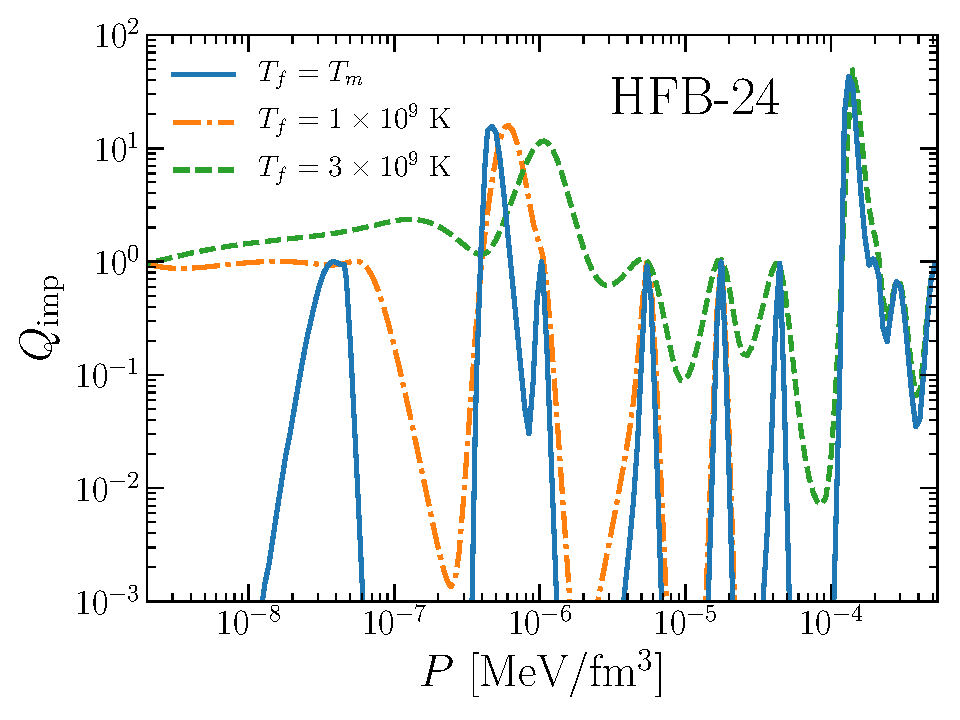
\includegraphics[width=0.9\linewidth]{figures/qimp_ocrust.pdf}
  \end{center}
  \caption[Impurity parameter versus pressure in the outer-crust regime]{
    Variation with pressure $P$ of the impurity parameter $Q_{\text{imp}}$,
    Eq.~(\ref{eq:qimp}), in the regime of the outer crust for three selected
    temperatures at which the composition is assumed to be frozen: 
    $T_f=T_m$ (solid blue line),
    $T_f=1\times 10^9$ \si{\kelvin} (dashdotted orange line), and 
    $T_f=3\times 10^9$ \si{\kelvin} (dashed green line).
    Experimental data are supplemented with masses from the microscopic 
    HFB-24 theoretical mass table~\cite{Goriely2013}. 
  Figure inspired from~\cite{Fantina2020}.}\label{fig:qimp_ocrust}
\end{figure}

% presentation of the figure
In Fig.~\ref{fig:qimp_ocrust}, the impurity parameter $Q_{\text{imp}}$ is 
plotted as a function of the pressure in the regime of the outer crust. As
previously, we make use of the microscopic HFB-24 theoretical mass
table~\cite{Goriely2013} to complement the present day experimental
information on nuclear masses~\cite{Huang2017,Welker2017}.
% we assume different values at which the composition is frozen
We recall that, considering the present uncertainties on timescales relative to 
NS cooling~\cite{Goriely2011}, the ion distribution could be frozen at some
temperature higher than $T_m$.
For this reason, we consider three different temperatures at which the 
composition could potentially freeze: $T_f = T_m$ (solid blue line), 
$T_f = 1\times 10^9$ K (dashdotted orange line), and $T_f = 3\times 10^9$ K 
(dashed green line).
For a given pressure, it is seen that the impurity factor tends to be larger as 
the temperature is increased.
Low values of $Q_{\text{imp}}$ indicate that the distribution $p(Z)$, see
Fig.~\ref{fig:pj_ocrust}, is strongly peaked on one particular nucleus. In that 
case, the OCP approximation is reliable. This is for instance
seen at low pressure for $T_f = T_m$. Conversely, the impurity parameter 
can reach values as high as $\approx 50$ around $P=1.5\times 10^{-4}$ 
MeV/fm$^3$ where the charge distribution exhibits a multimodal 
character. 
Strong oscillations of $Q_{\text{imp}}$ are observed due to shell structure
effects, suggesting that the outer crust is constituted of an alternation of 
highly resistive and highly conductive layers. This was originally observed
by Fantina \textit{et al.}~\cite{Fantina2020}, and we have checked 
that this conclusion is not sensitive to the model, as far as state-of-the-art
theoretical mass tables are used to complement experimental data.

\subsection{Abundancies of odd nuclei}\label{subsec:odd_ocrust}

In the original calculation of the outer-crust ground state at zero 
temperature, the possibility of having odd-mass or odd-charge nuclei was not 
envisaged due to nuclear pairing~\cite{BPS}.
However, using the HFB-24 mass model, a thin layer of odd-mass $^{121}$Y is 
observed at high pressure in the outer crust, see Table~\ref{table:ocrust}.
One can therefore expect the MCP mixture to be composed of several odd nuclei
at finite temperature.
%
The presence of unpaired nucleons in the outer crust could lead to
ferromagnetic phase transitions at low temperature, which in return could 
generate a magnetic field and alter the existing one, and so affect the 
electron gas. The importance of those effects depends on the spin and global
abundancy of odd nuclei.
%
Related quantities of interest are the fraction 
$\mathcal{N}_{\text{odd}}/\mathcal{N}$ and baryonic mass fraction 
$M_{B,\text{odd}}/M_B$ of odd nuclei in the outer crust, which can be evaluated 
once the abundancies of odd-$A$ and odd-$Z$ nuclei are computed for all 
pressures in the outer crust.
 
\begin{figure}[!t]
  \begin{center}
    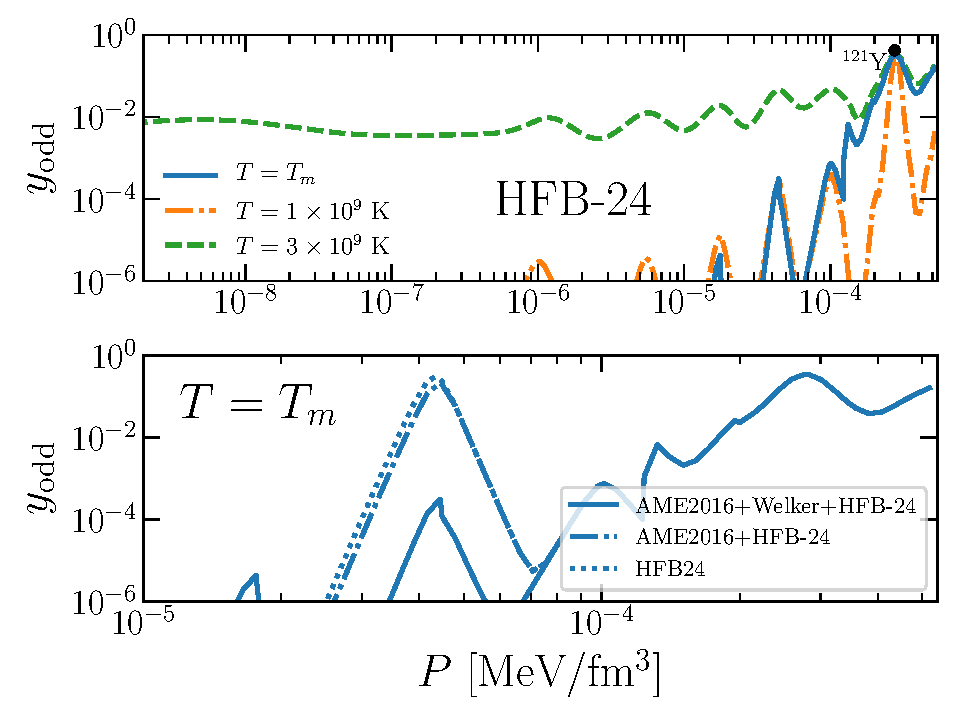
\includegraphics[width=0.9\linewidth]{figures/yodd_ocrust.pdf}
  \end{center}
  \caption[Fraction of odd-$A$ and odd-$Z$ nuclei versus pressure in the outer 
  crust regime]{
    Upper panel: Variation with pressure $P$ of the fraction of odd-$A$ and 
    odd-$Z$ nuclei $y_{\text{odd}}$, Eq.~(\ref{eq:yodd}), in the regime of the 
    outer crust for three selected
    temperatures: $T=T_m$ (solid blue line),
    $T=1\times 10^9$ \si{\kelvin} (dashdotted orange line), and 
    $T=3\times 10^9$ \si{\kelvin} (dashed green line).
    Experimental data are supplemented with masses from the microscopic 
  HFB-24 theoretical mass table~\cite{Goriely2013}. Lower panel:
$y_{\text{odd}}$ as a function of $P$ in the deepest layers of the outer crust
at the crystallization temperature, using three different mass tables:
AME2016+Welker+HFB-24 (solid line), AME2016+HFB-24 (dashdotted line), and
HFB-24 (dotted line).}\label{fig:yodd_ocrust}
\end{figure}

The fraction of odd-$A$ and odd-$Z$ nuclides in a given thermodynamic condition 
$(P,T)$ is obtained from the probabilities $p_j$ through
%
\begin{equation}
  y_{\text{odd}} = \frac{\sum_{j} p_j \delta_{\text{odd}}}{\sum_j p_j} 
  = \sum_j p_j\delta_{\text{odd}},\label{eq:yodd}
\end{equation}
%
with
%
\begin{eqnarray}
  \delta_{\text{odd}} =\left\{
                \begin{array}{ll}
                  1, \quad \text{if $A^{(j)}$ or $Z^{(j)}$ odd}\\
                  0, \quad \text{if $A^{(j)}$ and $Z^{(j)}$ even}
                \end{array}
              \right..
\end{eqnarray}
%
The upper panel of Fig.~\ref{fig:yodd_ocrust} shows the variation with pressure 
of $y_{\text{odd}}$ in the regime of the outer crust at the crystallization
temperature, (solid blue line), $T=1\times 10^9$ K (dashdotted orange 
line), and $T=3\times 10^9$ K (dashed green line). The HFB-24 mass table is
used to complement the available experimental masses.
We can see that more odd-mass and odd-charge nuclei are present in the outer
crust as the temperature is increased, because the influence of pairing
decreases with temperature. 
The fraction of odd-nuclei at crystallization is negligible, except in the
deepest layers of the outer crust where oscillations of $y_{\text{odd}}$ are
observed.
In particular, a remarkable peak, $y_{\text{odd}} = 0.42$, can be seen around 
$P = 2.75\times 10^{-4}$ MeV/fm$^3$, the most probable nucleus being $^{121}$Y.

The influence of the mass table on the fraction of odd nuclei present in the 
bottom layers of the outer crust at crystallization is investigated in the 
lower panel of Fig.~\ref{fig:yodd_ocrust}.
It is observed that $y_{\text{odd}}$ is very sensitive to the mass excesses of 
copper isotopes $^{77-79}$Cu in the vicinity of $P = 5\times 10^{-5}$ 
MeV/fm$^3$, and ranges from $\approx 4\times 10^{-4}$ (with mass excesses taken 
from~\cite{Welker2017}) to $\approx 0.35$ (with HFB-24 mass excesses).
Such difference highlights the fact that measuring masses of odd nuclei is 
important.

The fraction of odd nuclei contained in the outer crust is computed as
%
\begin{equation}
  \frac{\mathcal{N}_{\text{odd}}}{\mathcal{N}} =
  \frac{\int_{R=R'}^\infty d\mathcal{N}_{\text{odd}}(r)}
  {\int_{R=R'}^\infty d\mathcal{N}(r)},
\end{equation}
%
where $R'$ is the \edit{radial coordinate at the bottom of the outer crust}, 
and therefore depends on the imposed central density $\rho_c$. The number 
of (odd) nuclei contained in the elementary volume $dV(r)=4\pi r^2 dr$ is given 
by $d\mathcal{N}(r) = dV(r)n(r)$ ($d\mathcal{N}_{\text{odd}} 
= dV(r)n_{\text{odd}}(r)$), with $n(r) = 1/\langle V_{WS}\rangle$
($n_{\text{odd}} = \sum_j p_j \delta_{\text{odd}} /\langle V_{WS}\rangle$).
%
Similarly, the baryon mass fraction of odd nuclei is defined as
%
\begin{equation}
  \frac{M_{B,\text{odd}}}{M_B} =
  \frac{\int_{R=R'}^\infty dm_{\text{odd}}(r)}
  {\int_{R=R'}^\infty d{m}(r)}.
\end{equation}
%
The baryon mass of (odd) nuclei in the elementary volume $dV$ is given by
$dm(r) = dV(r)\rho_B(r)$ ($dm_{\text{odd}} = dV(r)\rho_{B,\text{odd}}$), with
the baryon mass density $\rho_B \propto \sum_j p_j F_i^{(j)}/\langle
V_{WS}\rangle$ ($\rho_{B,\text{odd}} \propto \sum_j 
p_j\delta_{\text{odd}}F_i^{(j)}/\langle V_{WS}\rangle$).
%
\begin{table}
  \begin{center}
    \begin{tabular}{ccc} 
      \toprule
      \toprule
      $T$ ($10^9$ K) & $\mathcal{N}_{\text{odd}}/\mathcal{N}$ ($\%$) & 
      $M_{B,\text{odd}}/M_B$ ($\%$)\\
      \midrule
      $T_m$ & 2.05 & 2.40\\
      $1.0$ & 2.30 & 2.65\\
      $2.0$ & 4.70 & 5.35\\
      \bottomrule
      \bottomrule
    \end{tabular}
  \end{center}
  \caption[Value of the fraction and baryon mass fraction of odd nuclei in the
  outer crust for three selected temperatures]{Value of the fraction of odd 
    nuclei $\mathcal{N}_{\text{odd}}/\mathcal{N}$ and baryon mass fraction of 
    odd nuclei $M_{B,\text{odd}}/M_B$ in the outer crust for three selected 
  temperatures. 
  Experimental data are supplemented with masses from the microscopic 
  HFB-24 theoretical mass table~\cite{Goriely2013}.}\label{table:oddnuc} 
\end{table}
%
We report our estimation of the fraction and baryon mass fraction of odd-$A$
and odd-$Z$ nuclei in the outer crust at crystallization,
$T=1\times 10^9$ K, and $T=2\times 10^9$ K in Table~\ref{table:oddnuc}. At the
crystallization temperature, we find that odd nuclei constitute $2.05\%$ of 
species in the outer crust and contribute $2.40\%$ of the outer-crust baryonic 
mass.

\section{Study of the inner crust at crystallization}\label{sec:icrust_tm}

While slightly softened with respect to CCM, shell effects in the outer 
crust at crystallization are still very important and are clearly reflected on 
the impurity parameter $Q_{\text{imp}}$, see Fig.~\ref{fig:qimp_ocrust}. 
Since the crystallization temperature increases with increasing depth, one can
wonder whether the shell corrections can be neglected in the free neutron
regime.
%
The composition of the inner crust is strongly model dependent due to the 
presence of an external neutron gas, thus the problem of the model dependence 
of the impurity factor naturally arises.

In this section, we present the results for the inner crust at finite
temperature, and more specifically at crystallization, using the CLD approach
developed in Chapter 1 with parameters optimized on four different microscopic
models, namely BSk22, BSk24, BSk25, and BSk26, introduced 
in~\cite{Goriely2013}.
As in Section~\ref{sec:ocrust_tm}, all thermal corrections introduced in
Section~\ref{sec:modelcrusttemp} are included in the ion free energy, unless
explicitly specified.
The highest average baryon density considered in this section is $n_B = 0.04$
fm$^{-3}$. Above this value, the presence of nonspherical pasta phases,
see~\ref{subsec:pasta}, is expected at finite temperature.
The influence of shell effects at the crystallization temperature is 
settled within the OCP approximation in~\ref{subsec:shtemp}.
In~\ref{subsec:mcp_results}, the equilibrium 
composition of the MCP mixture is presented, and the importance of the 
rearrangement term is investigated. Finally, the EoS dependence of the 
impurity parameter is explored.

\subsection{Influence of shell effects in the OCP
approximation}\label{subsec:shtemp}

In~\ref{subsec:strutinsky}, we have proposed a strategy to add perturbatively 
proton shell corrections to the CLD energy in the free neutron
regime. Let us recall that neutron shell effects become vanishingly small 
beyond the neutron-drip point~\cite{Chamel2006,Chamel2007}.
Strutinsky proton shell corrections have been tabulated in the inner 
crust at zero temperature for four recent functionals of the BSk family, namely 
BSk22, BSk24, BSk25, and BSk26~\cite{Pearson2018}. In the following, we 
introduce an empirical temperature-dependent factor to the zero-temperature 
shell corrections in the CLD free energy, before studying the influence of 
shell effects and exploring the model dependence of the inner-crust properties 
at the crystallization temperature.

\subsubsection{Temperature dependence of shell corrections}

\begin{figure}[!t]
  \begin{center}
    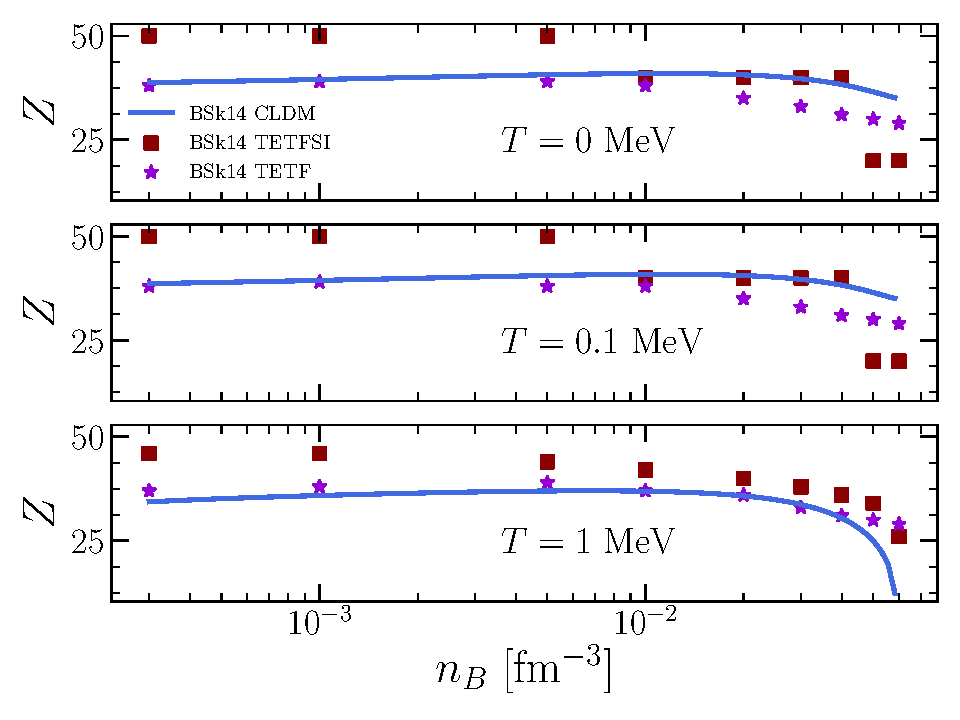
\includegraphics[width=0.9\linewidth]{figures/bsk14compo_vs_nb.pdf}
  \end{center}
  \caption[Equilbrium value of proton number versus baryon density in the inner
  crust for BSk14 at finite temperature]{Equilibrium value of proton number $Z$ 
    as a function of baryon density $n_B$ in the inner crust for the BSk14 
    functional for different temperatures: $T=0$ \si{\MeV} (upper panel), 
    $T=0.1$ \si{\MeV} (middle panel), and $T=1$ \si{\MeV} (lower panel). Solid 
    lines correspond to the 
    CLD model calculations without shell effects, and square (star) symbols 
    correspond to the TETFSI (TETF) results from~\cite{Onsi2008}. Figure 
    adapted from~\cite{Carreau2019}.}\label{fig:bsk14compo_vs_nb}
\end{figure}

The total free energy per ion including shell corrections in the crust reads
%
\begin{equation}
  F(n_B,Z,T) = F^{\text{CLD}}(n_B,Z,T) + E_{sh}(n_B,Z) 
  - TS_{sp}(n_B,Z,T),
\end{equation}
%
where $E_{sh}$ is the interpolated Strutinsky shell energy at $T=0$ K
(see~\ref{subsec:strutinsky}), and $S_{sp}$ the entropy responsible of the 
softening of shell effects at finite temperature. 
In the zero temperature limit, we want to recover 
$F(T=0) = E^{\text{CLD}}(T=0) + E_{sh}$, whereas at high
temperature shell effects should vanish, $F \rightarrow 
F^{\text{CLD}}$, yielding
%
\begin{equation}
  \lim_{T\rightarrow \infty} T S_{sp}(n_B,Z,T) = E_{sh}(n_B,Z).
\end{equation}
%
As a ansatz, we take
%
%\begin{equation}
%  TS_{sp} = \frac{2}{\pi}E_{sh}(n_B,Z)\arctan(\lambda T),
%\end{equation}
%%
%allowing us to rewrite the free energy per ion including temperature-dependent 
%shell corrections as
%
\begin{equation}
  F = F^{\text{CLD}} + E_{sh}(n_B,Z)\xi(T),
\end{equation}
%
the temperature-dependent factor being given by
%
\begin{equation}
  \xi(T) = \left(1-\frac{2}{\pi}\arctan(\lambda T)\right).
\end{equation}
%
The coefficient $\lambda$ can thus be determined by two parameters, $T_0$ and
$\xi_0 = \xi(T_0)$, such that
%
\begin{equation}
  \lambda = \frac{1}{T_0}\tan\left(\frac{\pi}{2}(1-\xi_0)\right).
\end{equation}
%
This is obviously a very rough treatment of the temperature dependence of shell 
effects, but we will show in~\ref{subsubsec:cryst_bsk} that the difference in 
the results obtained with or without this temperature dependence is smaller 
than the uncertainty due to our imperfect knowledge of the \edit{CLD} part of 
the nuclear functional.
 
A reasonable choice consists in adjusting $T_0$, corresponding to the 
temperature at which shell effects are wiped out, and $\xi_0$, which governs
the drop of $\xi$ with temperature, so as to reproduce the TETFSI results of 
Onsi \textit{et al.} for the equilibrium value of $Z$ in the inner crust using 
the BSk14 functional~\cite{Onsi2008} (see their Tables III and IV), 
represented in Fig.~\ref{fig:bsk14compo_vs_nb}, along with the results obtained 
with our CLD modeling for the same interaction.
As expected, it is seen that shell effects decrease as temperature is
increased, and that the discontinuous behavior of $Z$ persists 
until \edit{$T\approx 1$~{MeV} $\approx 1.2\times 10^{10}$~K}, when the TETFSI 
results follow the same smooth trend as the TETF and CLDM predictions.
Based on these considerations, we fix the two parameters to $T_0 = 1$ MeV and 
$\xi_0 = 0.02$.
An excellent agreement is observed between the CLDM and
TETF results -- for which proton shell corrections are also neglected -- at 
relatively high temperature. 
Let us remark that higher values of $Z$ are obtained in the 
CLD calculations than in the TETF ones at low temperature and high density,
which shows the limit of the CLD approach. 

\begin{figure}[!t]
  \begin{center}
    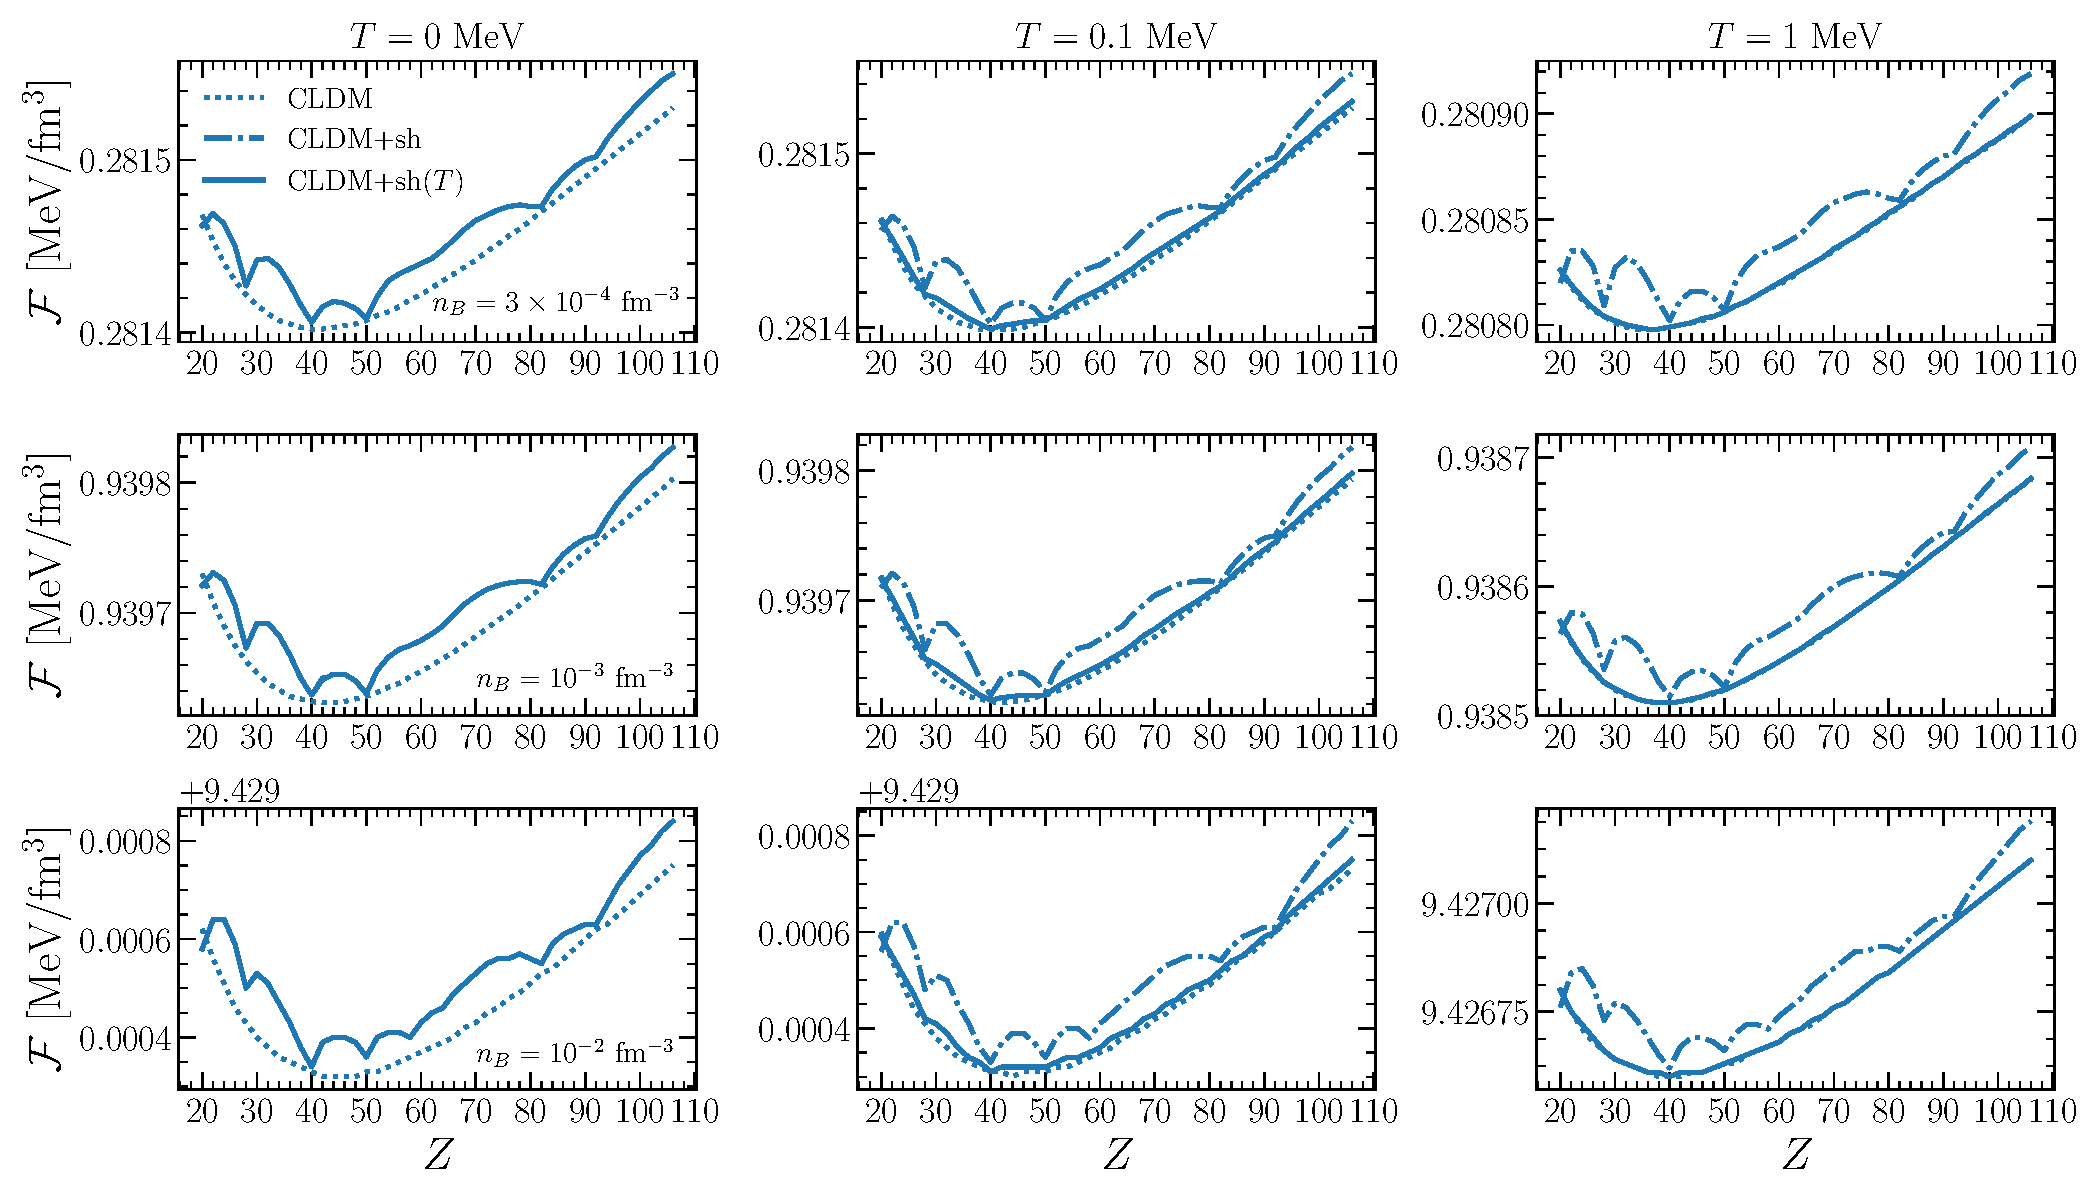
\includegraphics[width=1.0\linewidth]{figures/fdensws_vs_zz.pdf}
  \end{center}
  \caption[Free energy density versus proton number $Z$ for different
  thermodynamic conditions in the free neutron regime]{Free energy density as a 
    function of the proton number $Z$ for BSk24 CLDM for temperatures $T=0$ 
    \si{\MeV} (left panels), $T=0.1$ \si{\MeV} (central panels), and 
    $T=1$ \si{\MeV} (right panels), and baryon densities $n_B=3\times 10^{-4}$ 
    \si{\per \cubic\femto\meter} (upper panels), $n_B = 10^{-3}$ 
    \si{\per \cubic\femto\meter} (middle panels), and $n_B = 
    10^{-2}$ \si{\per \cubic\femto\meter} (lower panels). 
    In each panel, dashdotted (solid) lines correspond to the calculations
including temperature-independent (temperature-dependent) shell corrections,
and dotted lines represent the results without shell effects. Figure adapted
from~\cite{Carreau2019}.}\label{fig:fdensws_vs_zz}
\end{figure}
%
Fig.~\ref{fig:fdensws_vs_zz} shows the WS cell free energy density as a
function of the proton number $Z$ for different conditions of density
and temperature in the free neutron regime, for BSk24 CLDM with and without
temperature-independent (temperature-dependent) shell corrections.
%
The right panels show the results at zero temperature, 
which have been already discussed in in Fig.~\ref{fig:shcorr_bsk24}. The free
energy density with temperature-dependent and zero-temperature shell
corrections perfectly coincide since $\xi = 1$ for $T=0$ MeV.
%
We can clearly see that shell corrections are softened by the 
temperature-dependent factor at finite temperature (central and right panels). 
At the intermediate value $T=0.1$ MeV, we can appreciate the large 
difference between the free energy density with zero-temperature Strutinsky
shell corrections and that including temperature-dependent shell corrections
through the factor $\xi(T)$. Let us recall that this difference is sensitive to
the value of $\xi_0$.
%
We recover the expected behavior that nonsmooth effects are fully wiped out at 
$T=1$ MeV, corresponding to $\xi=0$. In that case, the pure CLD prediction is 
therefore equivalent to that accounting for temperature-dependent shell 
corrections.

\subsubsection{Equilibrium composition of the OCP at crystallization for modern 
BSk functionals}\label{subsubsec:cryst_bsk}

% intro figure
In the free neutron regime, the model dependence arises from the lack of 
experimental and theoretical constraints for very neutron rich nuclei and 
nuclear matter. 
This concerns the bulk properties, that is the nuclear EoS of asymmetric 
matter, but also surface properties, more specifically the surface tension of 
extremely neutron rich nuclei. 
% explain calculation
In Fig.~\ref{fig:tm_compo_final1}, we investigate the relative 
weight of the bulk and surface properties in determining the uncertainties in 
the crystallization temperature of a OCP (upper panel) and the corresponding 
equilibrium value of the ion atomic number $Z$ (lower panel).
These inner-crust properties are calculated for BSk22, BSk24, and BSk25
functionals within the CLD approximation, up to $n_B = 0.04$ fm$^{-3}$. 
Dashdotted lines correspond to 
the calculations in which surface and curvature parameters are fitted to 
experimental masses of 9 spherical and semimagic nuclei only, namely 
$^{40,48}$Ca, $^{48,58}$Ni, $^{88}$Sr, $^{90}$Zr, $^{114,132}$Sn, and 
$^{208}$Pb, while solid lines show the predictions with surface properties 
being fitted to the associated ETF calculations performed up to the 
respective neutron-drip lines~\cite{PearsonPriv} (default option). 
Let us notice that in both 
cases, the isovector surface parameter is fixed to the value $p=3$, which 
ensures a good reproduction of the CC transition density and pressure for each 
considered BSk functional~\cite{Carreau2019}.
The resulting predictions then differ solely in their bulk properties, and the
width of the gray bands can therefore be interpreted as an estimate of the 
uncertainty on $T_m$ and $Z$ arising from our incomplete knowledge of the 
nuclear EoS of asymmetric matter.
% discuss and interpret the results
In the upper panel, it is observed that higher values of the OCP ion atomic 
number $Z$ are obtained when surface tension of neutron-rich nuclei is adjusted 
on the microscopic ETF results, and of course this difference reflects on the 
crystallization temperature of the OCP (lower panel), which roughly scales as 
$Z^{5/3}$ according to the approximation Eq.~(\ref{eq:tmapprox}).
%
One should stress that the bulk 
parameters of the considered BSk functionals were precisely fitted to the 
properties of finite nuclei and \textit{ab initio} neutron-matter 
calculations~\cite{Goriely2013}. The residual uncertainty in the nuclear EoS is 
not negligible, but its consequence is less important than the uncertainties on 
the surface energy for neutron-rich nuclei close to neutron drip. The latter 
can then be considered as the key physical quantity determining the crust 
composition and crystallization temperature.
%
Given the present CLD calculations, we find that the crystallization 
temperature of a OCP in the inner crust ranges from $\approx 3\times 10^9$ K at 
the neutron-drip point to $\approx 9\times 10^9$ K at high density close to the 
CC transition point.
The different functionals lead to predictions that progressively diverge 
with increasing depth, the crystallization temperature differing by up to 
$40\%$ at the highest density considered.
The anticorrelation between the symmetry energy and the crystallization
temperature is clearly observed in the regime of the inner crust: the higher 
the symmetry energy at saturation, the lower the crystallization temperature, 
with $E_{sym}=32$ MeV, $E_{sym}=30$ MeV, and $E_{sym}=29$ MeV for BSk22, 
BSk24, and BSk25, respectively. The same is true for the equilibrium value of
$Z$, which is as in CCM $\approx 40$ all along the inner crust when 
surface properties are optimized on microscopic ETF calculations.
%
\begin{figure}[!t]
  \begin{center}
    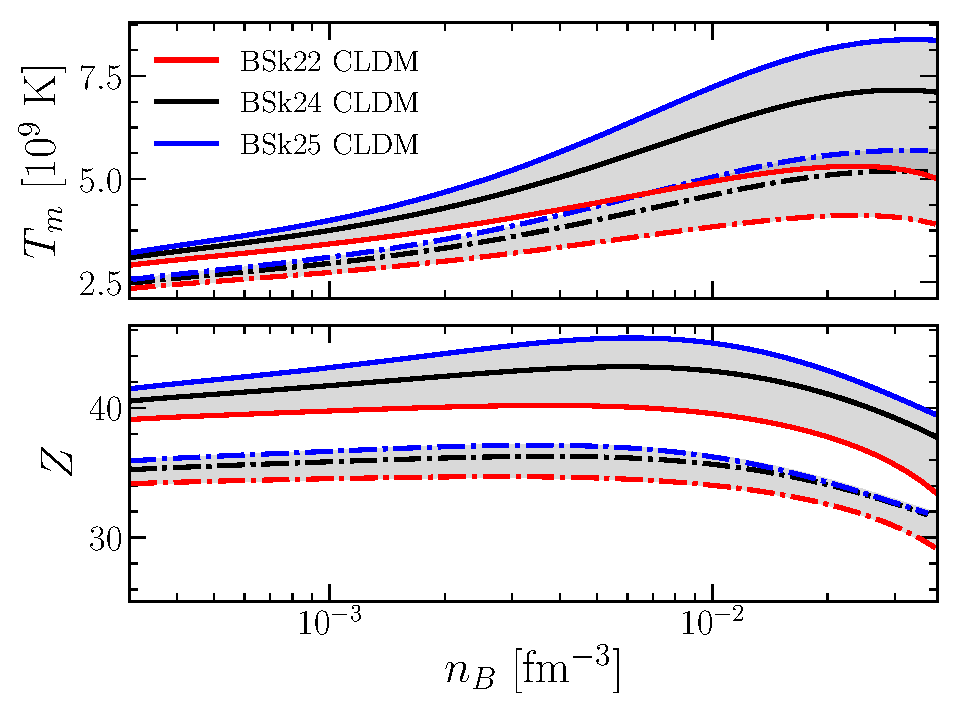
\includegraphics[width=0.9\linewidth]{figures/tm_compo_final1.pdf}
  \end{center}
  \caption[Crystallization temperature and equilibrium value of $Z$ of the
  one-component plasma versus baryon density in the inner crust]{
    Crystallization temperature $T_m$ (upper panel) and
    equilibrium value of $Z$ (lower panel) as a function of baryon density 
    $n_B$ in the inner crust for BSk22, BSk24, and BSk25 CLDM with surface and
  curvature parameters fitted to spherical nuclei (dashdotted lines), or to
associated ETF calculations (solid lines). Gray bands represent extrema. Figure
adapted from~\cite{Carreau2019}.}\label{fig:tm_compo_final1}
\end{figure}
 
In Fig.~\ref{fig:tm_compo_final2}, we show the results obtained for the same 
CLDM, with temperature-independent (temperature-dependent) shell corrections as 
dashdotted (solid) lines. The gray bands corresponding to the pure CLD results 
with surface parameters optimized on ETF calculations are reported in both
panels.
It is seen that, apart from BSk25 under the extreme and quite unrealistic
hypothesis that shell effects are not affected by temperature, all calculations
including shell corrections fit in the CLD bands. 
Given our estimation of the parameters entering the temperature-dependent
factor, $T_0=1$ MeV and $\xi_0 =0.02$, we find that the discontinuous behavior 
of the equilibrium value of ion atomic number $Z$ is entirely smoothed out at 
the crystallization temperature in the inner crust.
For these reasons, the simple CLD modeling, in which nonsmooth effects are
neglected, could be sufficient to study the inner-crust properties at 
crystallization.
Within the MCP approach, neglecting proton shell corrections in the free 
neutron regime will have the positive impact of drastically reducing the 
computational time.
%
\begin{figure}[!t]
  \begin{center}
    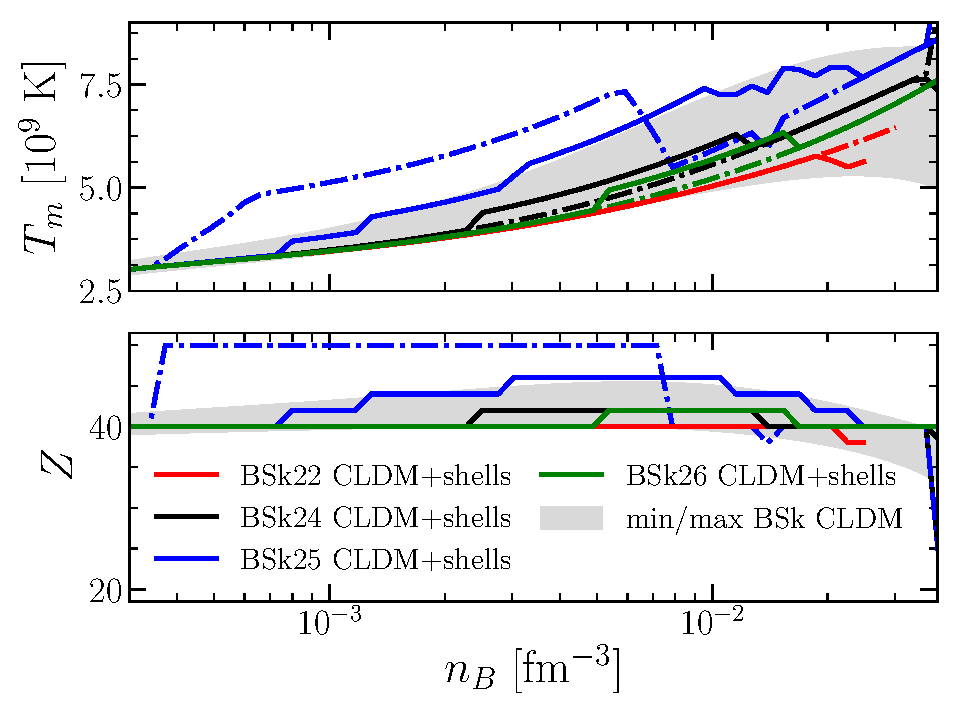
\includegraphics[width=0.9\linewidth]{figures/tm_compo_final2.pdf}
  \end{center}
  \caption[Crystallization temperature and equilibrium value of $Z$ of the
  one-component plasma versus baryon density in the inner crust]{
    Crystallization temperature $T_m$ (upper panel) and 
    equilibrium value of $Z$ (lower panel) as a function of baryon density 
    $n_B$ in the inner crust. The gray bands correspond to extrema for the 
    BSk22, BSk24, and BSk25 CLDM with surface parameters fitted to associated 
    ETF calculations. Solid (dashdotted) lines represent the calculations for 
    BSk22, BSk24, BSk25, and BSk26 CLDM with temperature-dependent 
    (temperature-independent) shell corrections. Figure adapted
    from~\cite{Carreau2019}.}\label{fig:tm_compo_final2}
\end{figure}

\begin{figure}[!t]
  \begin{center}
    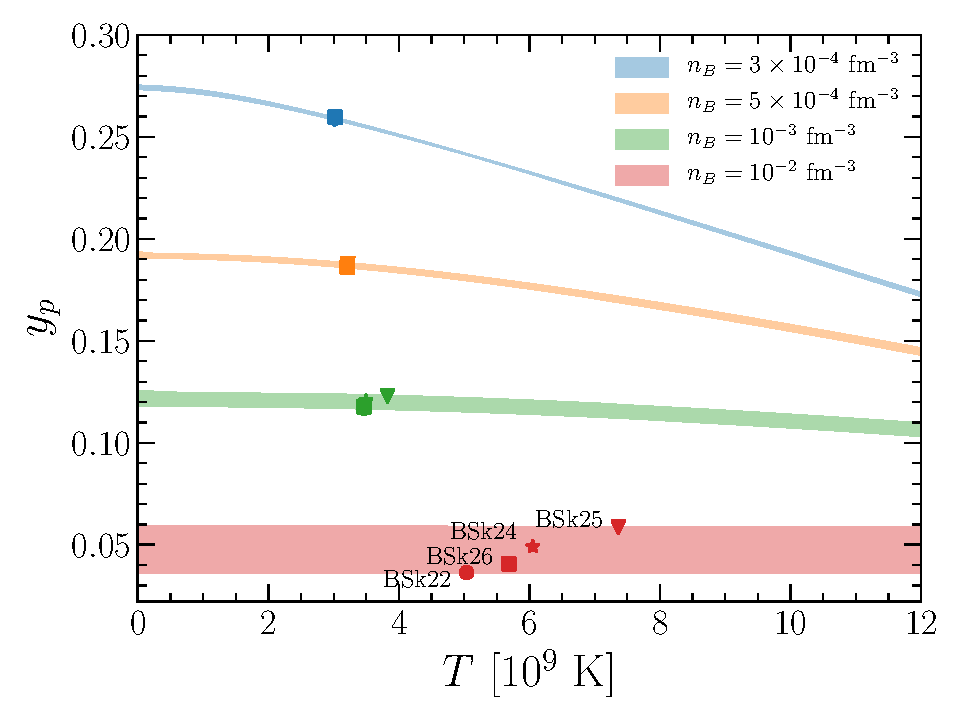
\includegraphics[width=0.9\linewidth]{figures/ypcell_ocp.pdf}
  \end{center}
  \caption[Equilibrium proton fraction of the one-component plasma versus
  temperature in the inner-crust regime]{Variation with temperature of the 
    equilibrium proton fraction of the OCP 
    for different values of the baryon density: $n_B = 3\times 10^{-4}$ 
    \si{\per \cubic\femto\meter} (blue band), $n_B = 5\times 10^{-4}$ 
    \si{\per \cubic\femto\meter} (orange band), $n_B = 10^{-3}$ 
    \si{\per \cubic\femto\meter} (green band), and $n_B = 10^{-2}$ 
    \si{\per \cubic\femto\meter} (red band). Each of the bands 
    represents extrema of pure CLD calculations for the four BSk functionals 
    including temperature-dependent shell corrections with $T_0 = 1$ \si{\MeV} 
    and $\xi_0 = 0.02$. Circles, stars, triangles, and squares indicate the 
    crystallization temperature for BSk22, BSk24, BSk25, and BSk26, 
    respectively. 
  Figure adapted from~\cite{Carreau2019}.}\label{fig:ypcell_ocp}
\end{figure}
%
Fig.~\ref{fig:ypcell_ocp} shows the proton fraction of the OCP at the 
equilibrium as a function of the temperature for four different baryon 
densities in the regime of the inner crust. 
For each value of $n_B$, the equilibrium proton fraction $y_p$ is calculated 
for BSk22, BSk24, BSk25, and BSk26 CLDM including temperature-dependent shell
corrections for $T$ up to $1.2\times 10^{10}$ K,
and a band is plotted to indicate the minima and maxima.
%
It is clearly seen that the band becomes thicker as we go deeper in the
star, showing that the model dependence of $y_p$ is more important at high 
density. 
The band associated to $n_B = 3\times 10^{-4}$ fm$^{-3}$, which is
very close to the neutron-drip point, is quite thin, reflecting the fact 
that the determination of the beta equilibrium is insensitive to the nuclear 
model employed at low density.
%
The fact that $y_p$ drops with temperature can be explained from the beta 
equilibrium equation $\mu_n - \mu_p = \mu_e$. Indeed, 
the electron chemical potential increases with temperature, yielding an 
increasing difference between the neutron and proton chemical potentials, and 
therefore a decreasing proton fraction.
%
While the CCM hypothesis appears to be well-founded in the inner-crust bottom 
layers, deviations at low density are observed with respect to the results at 
the crystallization temperature, which is indicated for each BSk functional.
%
As previously discussed, the composition of the crust could be frozen at some
temperature $T_f > T_m$ depending on the typical timescale of the weak
interaction relative to the cooling dynamics. In that case, and independently
of the nuclear model, the equilibrium proton fraction as obtained within the 
CCM hypothesis would be overestimated, and as a consequence the latter 
hypothesis would be challenged.
%
% The increased $Q$ value for neutron capture could alter the $r$-process that 
% is expected to take place in binary NS mergers. Further investigations are 
% desirable.

\subsection{MCP results}\label{subsec:mcp_results}

We now turn to present the results obtained within the MCP approach introduced
in~\ref{subsec:mcp}. 
%
The equilibrium composition of the MCP and the impurity parameter are
computed in the inner crust at the crystallization temperature and, for
comparison, at $T=1\times 10^{10}$ K, at which the MCP is in a liquid phase.
%
From~\ref{subsec:shtemp}, we have seen that the nonsmooth 
effects vanish in the inner crust at the crystallization temperature.
Therefore, all the results that we present in the following are based on pure
CLD calculations for BSk functionals, that is without including proton shell 
corrections. The surface and curvature parameters are fitted to the 
corresponding ETF calculations. 

\subsubsection{Equilibrium composition of the 
MCP}\label{subsubsec:mcp_compo_icrust}

\begin{figure}[!t]
  \begin{center}
    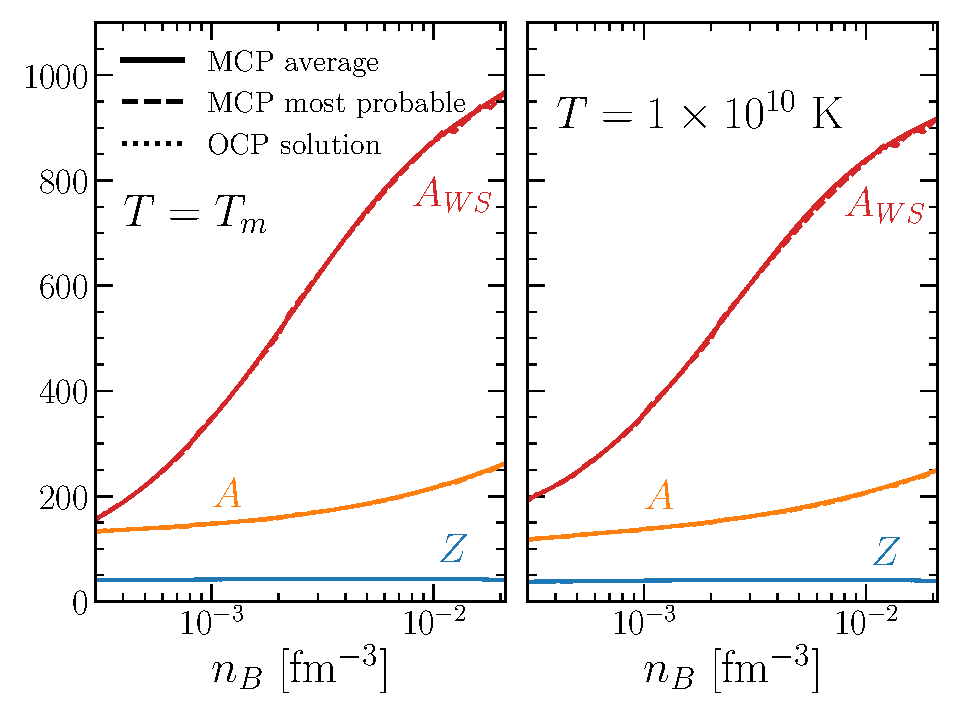
\includegraphics[width=0.9\linewidth]{figures/compo_icrust_bsk24_mcp.pdf}
  \end{center}
  \caption[Equilibrium composition of the multicomponent plasma versus
  baryon density in the inner-crust regime]{
    Average (solid lines) and most probable values (dashed lines) of the charge 
    number $Z$ (blue lines), cluster mass number $A$ (orange lines), and total
    mass number $A_{WS}$ (red lines) in the MCP mixture as a function of 
    the average baryon density in the regime of the inner crust at 
    $T=T_m$ (left panel) and $T=1\times 10^{10}$ \si{\kelvin} (right panel). 
    The OCP solution is represented in dotted lines.
    Figure adapted from~\cite{Carreau2020}.}\label{fig:compo_icrust_bsk24_mcp}
\end{figure}
%
The average (solid lines) and most probable value (dashed lines) of the proton 
number $Z$, cluster mass number $A$, and WS cell mass number $A_{WS}$ in the 
MCP mixture are plotted as a function of the average baryon density in the free 
neutron regime at crystallization (left panel) and at a higher temperature 
$T=1\times 10^{10}$ K (right panel) for the BSk24 CLDM.
%
It is observed that the MCP results are extremely close to the OCP ones, which 
are represented as dotted lines. This shows that, as in the regime of the outer 
crust~\cite{Fantina2020}, deviations with respect to the linear mixing rule are 
very small.
%
By comparing the results displayed in the two panels, we can see that the 
cluster mass and total mass increase as the temperature is decreased. 
%
As in the zero-temperature limit, see Fig.~\ref{fig:compo_icrust_bsk24}, the 
average value of the ion atomic number stays almost constant in the inner 
crust, $\langle Z\rangle \approx 40$.

\begin{figure}[!t]
  \begin{center}
    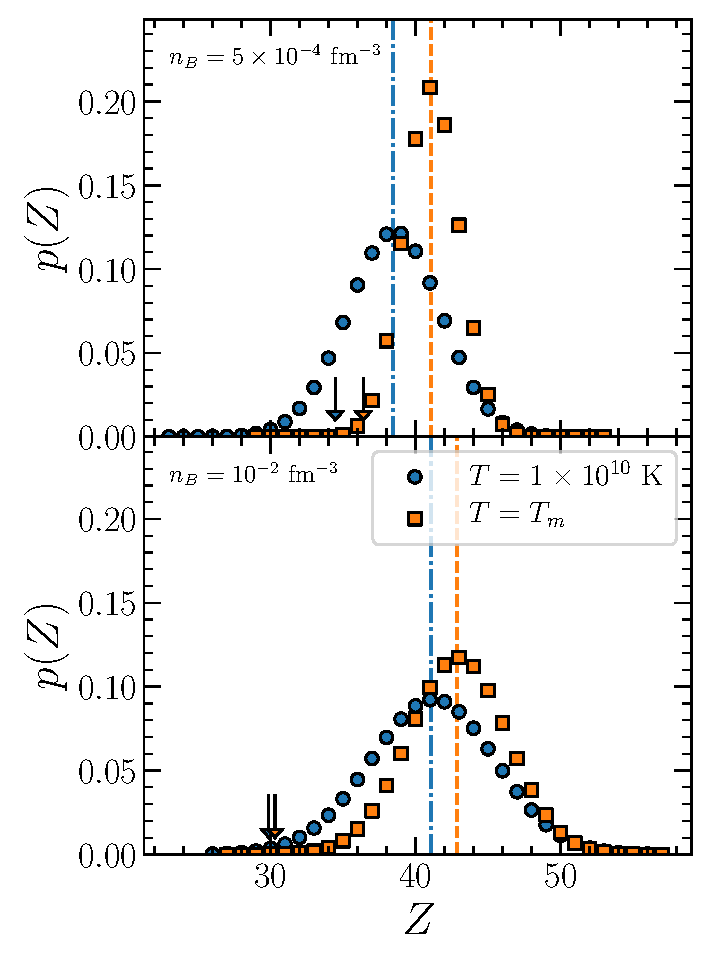
\includegraphics[width=0.49\linewidth]{figures/pj_icrust_bsk24.pdf}
    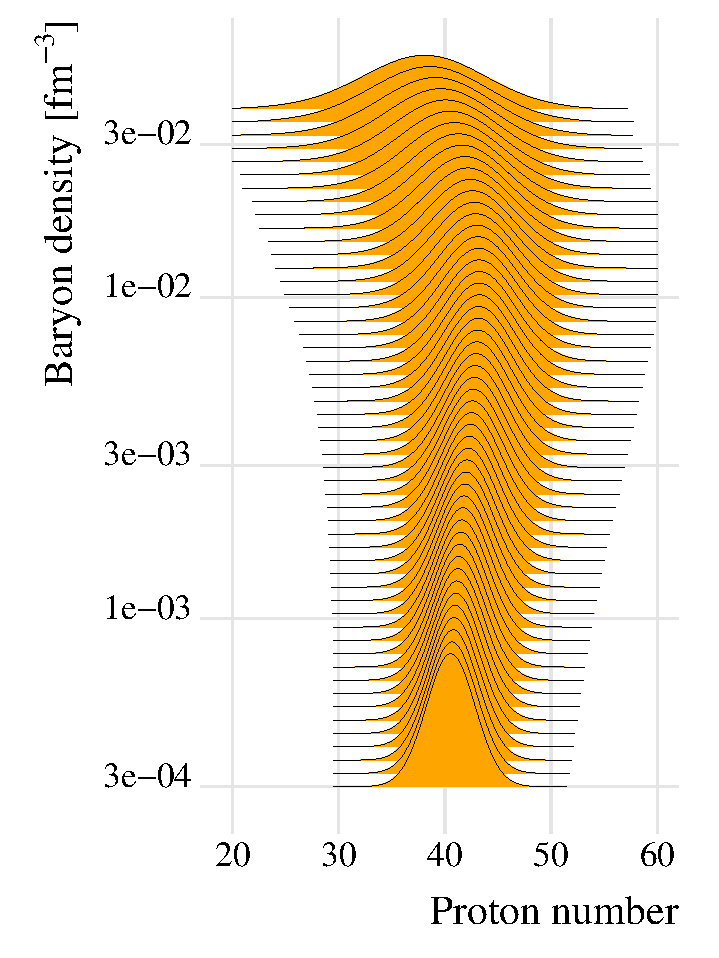
\includegraphics[width=0.49\linewidth]{figures/joyplot_bsk24_tm.pdf}
  \end{center}
  \caption[Normalized probability distribution of the atomic number $Z$ in the 
  inner-crust regime]{Left: Normalized 
    probability distribution 
    $p(Z)$ for $n_B=5\times 10^{-4}$ \si{\per \cubic\femto\meter} (upper
    panel) and $n_B=10^{-2}$ \si{\per \cubic\femto\meter} (lower panel), at 
    $T=1\times 10^{10}$ \si{\kelvin} (blue circles) and 
    $T=T_m$ (orange squares) for BSk24 CLDM. The blue dashdotted and orange 
    dashed vertical lines correspond to the respective OCP solutions, and 
    arrows indicate the value of $\langle Z\rangle$ without considering the 
    rearrangement term. Right: $p(Z)$ with increasing baryon density $n_B$ in 
    the inner crust at crystallization for BSk24 CLDM. Figure adapted 
  from~\cite{Carreau2020}.}\label{fig:pj_icrust}
\end{figure}
%
The left panels in Fig.~\ref{fig:pj_icrust} shows the normalized
probability distribution $p(Z)$ for $T=T_m$ (orange squares) and 
$T=1\times 10^{10}$ K (blue circles), and for
two selected values of the average baryon density in the inner-crust regime:
$n_B = 5\times 10^{-4}$ fm$^{-3}$ (top panel) and $n_B = 10^{-2}$ fm$^{-3}$
(bottom panel). The BSk24 CLDM is used.
%
Once again, the fact that the peaks of the distributions, that is the most
probable $Z$, coincides with the OCP solutions, represented by the vertical 
lines, shows that nonlinear mixing effects are negligible and thus 
that the linear mixing rule is a good approximation.
%
The importance of the rearrangement term, Eq.~(\ref{eq:rear}) can be 
appreciated by comparing, for each thermodynamic condition, the most probable
value of the ion atomic number with the average value obtained if the 
rearrangement term is not included in the calculation, indicated by the
corresponding arrow. Without including the rearrangement term, we observe a 
systematic and significant shift toward lower $Z$, showing that it is needed 
in order to ensure thermodynamic consistency. We can see that this effect
becomes more important as we go deeper in the inner crust. We stress that this 
term is not included in any of the NSE models which are presently available for 
astrophysical simulations. 
We can notice that, as expected, $p(Z)$ gets flatter as
density and temperature are increased, thus making the OCP approximation less
reliable. This is better demonstrated in the right panel of
Fig.~\ref{fig:pj_icrust}, which shows the variation with average baryon density 
of the normalized probability distribution $p(Z)$ in the inner crust at
crystallization.
It is seen that the distribution is peaked around $40$ throughout the inner
crust. At high density close to the CC transition, the range of $Z$ of the
distribution varies from $\approx 20$ up to $\approx 50$.

\subsubsection{Impurity parameter}\label{subsubsec:eos_qimp}

\begin{figure}[!t]
  \begin{center}
    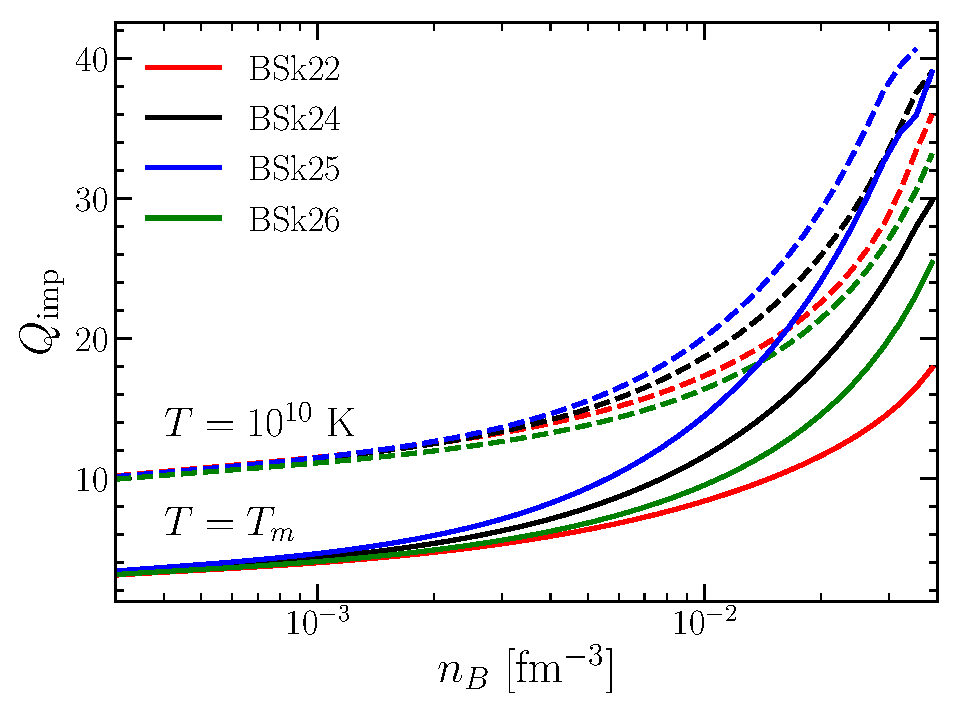
\includegraphics[width=0.9\linewidth]{figures/qimp_icrust.pdf}
  \end{center}
  \caption[Impurity parameter versus baryon density in the inner-crust 
  regime]{Variation with average baryon density $n_B$ of the impurity
    parameter $Q_{\text{imp}}$ in the regime of the inner crust for two
    selected temperatures: $T=T_m$ (solid lines) and $T=1\times 10^{10}$ 
    \si{\kelvin} (dashed lines), based on BSk22 (red lines), BSk24 (black 
    lines), BSk25 (blue lines), and BSk26 (green lines) CLD calculations.
    Figure published in~\cite{Carreau2020}.}\label{fig:qimp_icrust}
\end{figure}
%
In the inner crust, we have to address the problem of model dependence in 
order to make a quantitative prediction of the impurity parameter 
$Q_{\text{imp}}$. 
Apart from the modeling of finite temperature shell effects discussed 
thoroughly in~\ref{subsec:shtemp}, the main source of uncertainty 
of the calculation comes from the choice of the nuclear functional. We show, 
in Fig.~\ref{fig:qimp_icrust}, the impurity parameter, Eq.~(\ref{eq:qimp}), as 
a function of the average baryon density in the inner crust, at the 
crystallization temperature $T_m$ (solid lines), for the four considered BSk 
CLD models. 
Considering that the chosen models are believed to cover the main uncertainty 
on the nuclear EoS at subsaturation density~\cite{Pearson2018}, we can take the 
spread of $Q_{\text{imp}}$ values as obtained by the four calculations, as a 
reasonable estimation of the uncertainty on the impurity parameter. Since this 
latter represents the variance of the charge distribution, low values of
$Q_{\text{imp}}$ indicate that the distribution is quite peaked and thus that 
the OCP approach is a good approximation, as it can also be seen from
Figs.~\ref{fig:compo_icrust_bsk24_mcp} and~\ref{fig:pj_icrust}. In particular, 
the monotonic increase of the impurity parameter with baryon density is in 
aggreement with the right panel of Fig.~\ref{fig:pj_icrust}, which clearly show 
the growth of the width of the ion atomic number distribution with increasing 
density. 
%
While at lower densities all the models predict similar values of the impurity 
parameter, $Q_{\text{imp}} \lesssim 5$, at higher densities the spread among 
the models becomes larger, with the functional associated to the larger 
symmetry energy at saturation density $E_{sym}$ having the larger 
$Q_{\text{imp}}$, leading to a relative difference of $\approx 55\%$ at $n_B
= 0.04$ fm$^{-3}$. 
Let us recall that the obtained values of the impurity parameter represent a
lower limit. Indeed, larger values are expected in the presence of nonspherical
geometries and/or fast cooling dynamics. For this reason, we also represent the
impurity parameter for $T= 1\times 10^{10}$ K (dashed 
lines). At this value of temperature, the same trend is observed, although the 
hierarchy of the models is not preserved.

\section{Conclusions}\label{sec:conclu3}

In this chapter, we have considered the modeling of the crust at finite
temperature. 
The OCP approximation, in which the expected distribution of
nuclei is replaced by a single nucleus obtained from the minimization of the
thermodynamic potential at a given thermodynamic condition, has been reviewed.
We have given the expressions of the thermal corrections entering the ion 
free energy, namely the translational center-of-mass motion term in the liquid 
phase, the zero-point quantum vibrations term in the solid phase, and the 
Coulomb interaction contribution which differs according to the phase of 
matter. We have discussed the definition of the transition from liquid to
solid, and we have then included the nuclear distribution in an MCP approach at 
the equilibrium. 
Within this treatment, nonlinear mixing effects arise due to 
the fact that the center-of-mass position of each ion is not confined to the 
single WS cell volume but can freely explore the whole volume. This is well
known in the plasma literature under the term of ``mixing entropy''.
The neutron and proton chemical potentials in the MCP mixture were found to be 
very close to the OCP ones, showing that a perturbative implementation of the 
NSE is sufficient. 
We have seen that a rearrangement term enters the expression of thermodynamic 
potential due to the self-consistency induced by the Coulomb part of the ion 
free energy, and we have proposed an approximation of this term which avoids
solving a complex self-consistent problem, by imposing the most 
probable nucleus to coincide with the OCP solution in the OCP limit.
% nuclear modeling in the free neutron regime
As in the zero-temperature limit, we have chosen to use the CLD approach to 
model the nuclear free energy in the free neutron regime. 
Sommerfeld expansions, reliable at low temperature, have been employed to 
derive the expression of the nuclear matter free energy as well as chemical
potential of nucleons. Because of the low values of the crystallization 
temperature expected in the crust, we have safely neglected the excitation of 
surface modes.

Using experimental masses supplemented with state-of-the-art microscopic
theoretical mass tables, we have shown results relevant for the outer crust of
PNS, that is for low temperatures and more particularly at crystallization.
% ocrust tm
We have calculated the crystallization temperature of a OCP throughout the
outer crust. We have observed that neglecting the anharmonic contribution to 
the ion free energy in the solid phase lead to an underestimation of the
crystallization temperature, which ranges from approximately $5\times 10^7$ K 
at very low pressure to $2.8\times 10^9$ K in the vicinity of the neutron-drip 
point, and exhibits a discontinuous behavior due to the shell effects. 
We have verified that the crystallization temperature is not strongly 
dependent on the mass model in the bottom layers of the outer crust, as long as 
realistic theoretical mass tables are employed.
% ocrust compo
We have found that the composition of the outer crust at crystallization 
is very close to that calculated in the CCM hypothesis, and that the average
value of mass number $A$ and charge number $Z$ in the MCP mixture follow 
closely the equilibrium OCP solutions throughout the outer crust. 
As pressure and temperature are increased, we have shown that the charge 
distributions become broader, making the OCP approximation less reliable.
% ocrust qimp
We have computed the so-called impurity parameter $Q_{\text{imp}}$, which 
represents the variance of the charge distribution, at the crystallization 
temperature, and recovered the original results of~\cite{Fantina2020}.
Important oscillations of $Q_{\text{imp}}$ have been observed, suggesting that
the outer crust might consists of an alternation of highly resistive and 
highly conductive layers, and we have found that it can reach values as high as 
$\approx 50$ when the charge distribution exhibits a multimodal character.
% ocrust yodd
We have also evaluated the fraction of odd-mass and odd-charge nuclei present 
in the outer crust. We have shown that this quantity 
increases with temperature, and that, at crystallization, odd nuclei 
constitute $\approx 2\%$ of species in the outer crust, and contribute 
$\approx 2.4\%$ of the outer-crust baryonic mass. 

Finally, using the latest BSk functionals, we have presented results relevant 
for the inner crust of PNS, particularly at the crystallization temperature.
% icrust shells
Following our work at zero temperature, we have added temperature-dependent 
shell corrections to the CLD free energy, and within the OCP approximation, we 
have demonstrated that the highest source of model dependence of the 
crystallization temperature and associated composition comes from the smooth 
part of the nuclear functional. In addition, we have seen that shell 
effects are strongly softened at the crystallization temperature in the inner 
crust, which we have estimated to lie between $\approx 3\times 10^9$ K and 
$\approx 9\times 10^9$ K. 
Concerning the composition at crystallization, we have observed deviations with 
respect to CCM at low density. 
% icrust mcp
Within the MCP treatment, we have shown that at the crystallization temperature
the composition of the inner crust is dominated by clusters with charge number
$Z\approx 40$, while the range of the charge distribution varies from about 
$20$ near the neutron-drip point, to about $40$ close to the transition to
homogeneous matter.
This reflects on the behavior of the impurity parameter that monotonically 
increases with average baryon density up to around $40$ in the deeper regions 
of the inner crust.
We have also observed that the inclusion of the rearrangement term is required 
to guarantee thermodynamic consistency.

\clearpage\thispagestyle{empty}
